%!TEX TS-program = pdflatex                                          %
%!TEX encoding = UTF8                                                %
%!TEX spellcheck = en-US                                             %
%
%%%%%%%%%%%%%%%%%%%%%%%%%%%%%%%%%%%%%%%%%%%%%%%%%%%%%%%%%%%%%%%%%%%%%%
% Handout_ModelingStructuralLesions.tex
% A handout to follow during the hands-on session 3 
% 
% Author: Paula Sanz Leon
% 
% 
%%%%%%%%%%%%%%%%%%%%%%%%%%%%%%%%%%%%%%%%%%%%%%%%%%%%%%%%%%%%%%%%%%%%%%
% based on the tufte-latex template                                  %

\documentclass{tufte-handout}

%\geometry{showframe}% for debugging purposes -- displays the margins

\usepackage{amsmath}

% Set up the images/graphics \underline{\textbf{Analysis}}
\usepackage[pdftex]{graphicx}
\setkeys{Gin}{width=\linewidth,totalheight=\textheight,keepaspectratio}
\graphicspath{{figures/} {../../framework_tvb/tvb/interfaces/web/static/style/img/} {../../framework_tvb/tvb/interfaces/web/static/style/img/nav/}}

\title{The Virtual Brain: Hands on Session \#3}
\date{7th June 2014} 

% The following package makes prettier tables.  
\usepackage{booktabs}


% The units package provides nice, non-stacked fractions and better spacing
% for units.
\usepackage{units}
\usepackage[svgnames]{xcolor}

% The fancyvrb package lets us customize the formatting of verbatim
% environments.  We use a slightly smaller font.
\usepackage{fancyvrb}
\fvset{fontsize=\normalsize}

% Small sections of multiple columns
\usepackage{multicol}

% For adjustwidth environment
\usepackage[strict]{changepage}

% For formal definitions
\usepackage{framed}

% And some maths
\usepackage{amsmath}  % extended mathematics

% Resume a list
\usepackage{enumitem}

% Background image
\usepackage{wallpaper}

% Background
\usepackage{hyperref}


% Provides paragraphs of dummy text
\usepackage{lipsum}

% These commands are used to pretty-print LaTeX commands
\newcommand{\doccmd}[1]{\texttt{\textbackslash#1}}% command name -- adds backslash automatically
\newcommand{\docopt}[1]{\ensuremath{\langle}\textrm{\textit{#1}}\ensuremath{\rangle}}% optional command argument
\newcommand{\docarg}[1]{\textrm{\textit{#1}}}% (required) command argument
\newenvironment{docspec}{\begin{quote}\noindent}{\end{quote}}% command specification environment
\newcommand{\docenv}[1]{\textsf{#1}}% environment name
\newcommand{\docpkg}[1]{\texttt{#1}}% package name
\newcommand{\doccls}[1]{\texttt{#1}}% document class name
\newcommand{\docclsopt}[1]{\texttt{#1}}% document class option name

\newcommand\blfootnote[1]{\begingroup
         \renewcommand\thefootnote{}\footnote{\phantom{\thefootnote} #1}%
         \addtocounter{footnote}{-1}%
         \endgroup
          }

% Colours: environment derived from framed.sty: see leftbar environment definition
\definecolor{formalshade}{rgb}{0.95,0.95,1}
\definecolor{simulationshade}{rgb}{0.92, 1.0, 0.95}

% Title rule
\newcommand{\HRule}{\rule{\linewidth}{0.5mm}}

% Framed  coloured boxes

%% Blue box: for steps regarding analysis and such
\newenvironment{formal}{%
  \def\FrameCommand{%
    \hspace{1pt}%
    {\color{DarkBlue}\vrule width 2pt}%
    {\color{formalshade}\vrule width 4pt}%
    \colorbox{formalshade}%
  }%
  \MakeFramed{\advance\hsize-\width\FrameRestore}%
  \noindent\hspace{-4.55pt}% disable indenting first paragraph
  \begin{adjustwidth}{}{7pt}%
  \vspace{2pt}\vspace{2pt}%
}
{%
  \vspace{2pt}\end{adjustwidth}\endMakeFramed%
}

%% Green box: for steps regarding simulatio **only**
\newenvironment{simulation}{%
  \def\FrameCommand{%
    \hspace{1pt}%
    {\color{ForestGreen}\vrule width 2pt}%
    {\color{simulationshade}\vrule width 4pt}%
    \colorbox{simulationshade}%
  }%
  \MakeFramed{\advance\hsize-\width\FrameRestore}%
  \noindent\hspace{-4.55pt}% disable indenting first paragraph
  \begin{adjustwidth}{}{7pt}%
  \vspace{2pt}\vspace{2pt}%
}
{%
  \vspace{2pt}\end{adjustwidth}\endMakeFramed%
}

%% Orange box: for verbose descriptions
\newenvironment{blah}{%
  \def\FrameCommand{%
    \hspace{1pt}%
    {\color{DarkOrange}\vrule width 2pt}%
    {\color{PeachPuff}\vrule width 4pt}%
    \colorbox{PeachPuff}%
  }%
  \MakeFramed{\advance\hsize-\width\FrameRestore}%
  \noindent\hspace{-4.55pt}% disable indenting first paragraph
  \begin{adjustwidth}{}{7pt}%
  \vspace{2pt}\vspace{2pt}%
}
{%
  \vspace{2pt}\end{adjustwidth}\endMakeFramed%
}

\begin{document}
\thispagestyle{plain}
\LLCornerWallPaper{1.5}{background.png}
\begin{titlepage}
\begin{center}
% Upper part of the page. The '~' is needed because \\
% only works if a paragraph has started.

\includegraphics[width=1.5\textwidth]{./tvb_logo_transparent_square.png}~\\[0.5cm]

% Title
\begin{fullwidth}
\HRule \\[0.2cm]
\begin{center}
{ \huge \bfseries Hands-on Session \#3 \\ [0.2cm] Modelling Structural Lesions \\[0.1cm] }
{ \large \bfseries June 7, 2014 \\[0.2cm]}
\end{center}
\HRule \\[0.2cm]
\end{fullwidth}

\end{center}
\end{titlepage}
\newpage
\ClearWallPaper
\begin{abstract}
\noindent  Altered long-range connectivity and large-scale brain network dynamics are expected to shed light in characterizing and understanding the so-called network disorders. 
\begin{marginfigure}%
  %
\includegraphics[width=\linewidth]{tvb_logo_transparent_square}
  %\caption{TVB evil logo}
  \label{fig:marginfig}
\end{marginfigure}
\end{abstract}

%\begin{fullwidth} % uncomment this environment to get full texwidth paragraphs 
%\textsc{The Virtual Brain} is a facilitating technology. It enables
%researchers from the domains of  computational neuroscience and medicine to
%study and focus on a particular problem, and directly build a model of the
%brain that can be tested under different scenarios. So, every time we require
%to perform a simulation for our work, we do not require to develop the
%underlying computational model.   
%\end{fullwidth}

\section{Objectives}\label{sec:objectives}

\newthought{From a scientific point} of view, the aim is to obtain a better understanding of
how structural lesions can be characterized; and more specifically, how those
changes may modify the local fast dynamics of the neural activity, as well
as the impact on global lower time scales signals such as BOLD. The main goal of this
session is to provide a clear understanding of the available tools to explore, analyze and edit
a connectome. Furthermore, in addition to TVB's default connectivity matrix we will have two additional matrices, one of a control subject and the other from a stroke
patient.

\section{Project: Session\_III\_ModellingStructuralLesions}\label{sec:project_data}

\begin{margintable}
  \centering
  \fontfamily{ppl}\selectfont
  \begin{tabular}{l}
    \toprule
    Name                                              \\
    \midrule
    \multicolumn{1}{l}{Removing Interhemispheric Connections}\\
    \\
    \multicolumn{1}{l}{Removing Nodes Based On Network Metrics}\\
    \\
    \multicolumn{1}{l}{The Effect Of The Structural}\\
    \multicolumn{1}{l}{Connectivity On The Global Stability Map}\\
    \textit{NoInterhemispheric\_g2d\_pse}\\
    \textit{NoHighInStrength\_g2d\_pse}\\
    \textit{NoHighInDegree\_g2d\_pse}\\
    \textit{Default\_g2d\_pse}\\
     \\
	\multicolumn{1}{l}{Region-based Simulations Of A Control }\\
    \multicolumn{1}{l}{And Stroke Connectome}\\

    $\quad$\textit{Control\_g2d\_pse}           \\
    $\quad$\textit{Stroke\_g2d\_pse}             \\
    %$\quad$\textit{Control\_g2d\_init\_bold} \\
    %$\quad$\textit{Stroke\_g2d\_init\_bold}        \\  
    $\quad$\textit{Control\_g2d\_init\_bold\_branch1}           \\
    $\quad$\textit{Stroke\_g2d\_init\_bold\_branch1} \\ 
    \\
    \multicolumn{1}{l}{Region-based Simulations Of A Control  }\\
    \multicolumn{1}{l}{And Stroke Connectome Using}\\
    \multicolumn{1}{l}{A Higher-dimensional Model}\\
    $\quad$\textit{Control\_sj3d\_pse}\\
    $\quad$\textit{Stroke\_sj3d\_pse}\\
    %$\quad$\textit{Control\_sj3d\_init\_bold}\\
    %$\quad$\textit{Stroke\_sj3d\_init\_bold}\\
    $\quad$\textit{Control\_sj3d\_init\_bold\_branch1}\\
    $\quad$\textit{Stroke\_sj3d\_init\_bold\_branch2}\\
    \bottomrule
  \end{tabular}
  \caption{Simulations in this project.}
  \label{tab:normaltab}
\end{margintable}


% let's start a new thought -- a new section
\newthought{In this session}, because the execution times for BOLD simulations
are long (in the order of hours or days), we'll only go through the necessary
steps required to reproduce some of the simulations listed in
Table~\ref{tab:normaltab}. You can click along and/or try to change
parameters and relaunch the simulations.


\begin{blah}
\textsc{Figure}~\ref{fig:fig} shows one of the most prominent working areas in
\textsc{TVB}: the \underline{connectivity editor}. In the same working area,  several
visualizers are available for displaying the matrices (e.g \underline{Matrix} and \underline{Space-Time}); and some of them may use node-wise
metrics to set the colour and size of the nodes (e.g., \underline{Hemisphere 1}, \underline{Transverse} and \underline{Hemisphere 2}). If you do not select any
metric before launching the connectivity editor, you can always set these
properties later.
\end{blah}

\begin{figure}[h]
  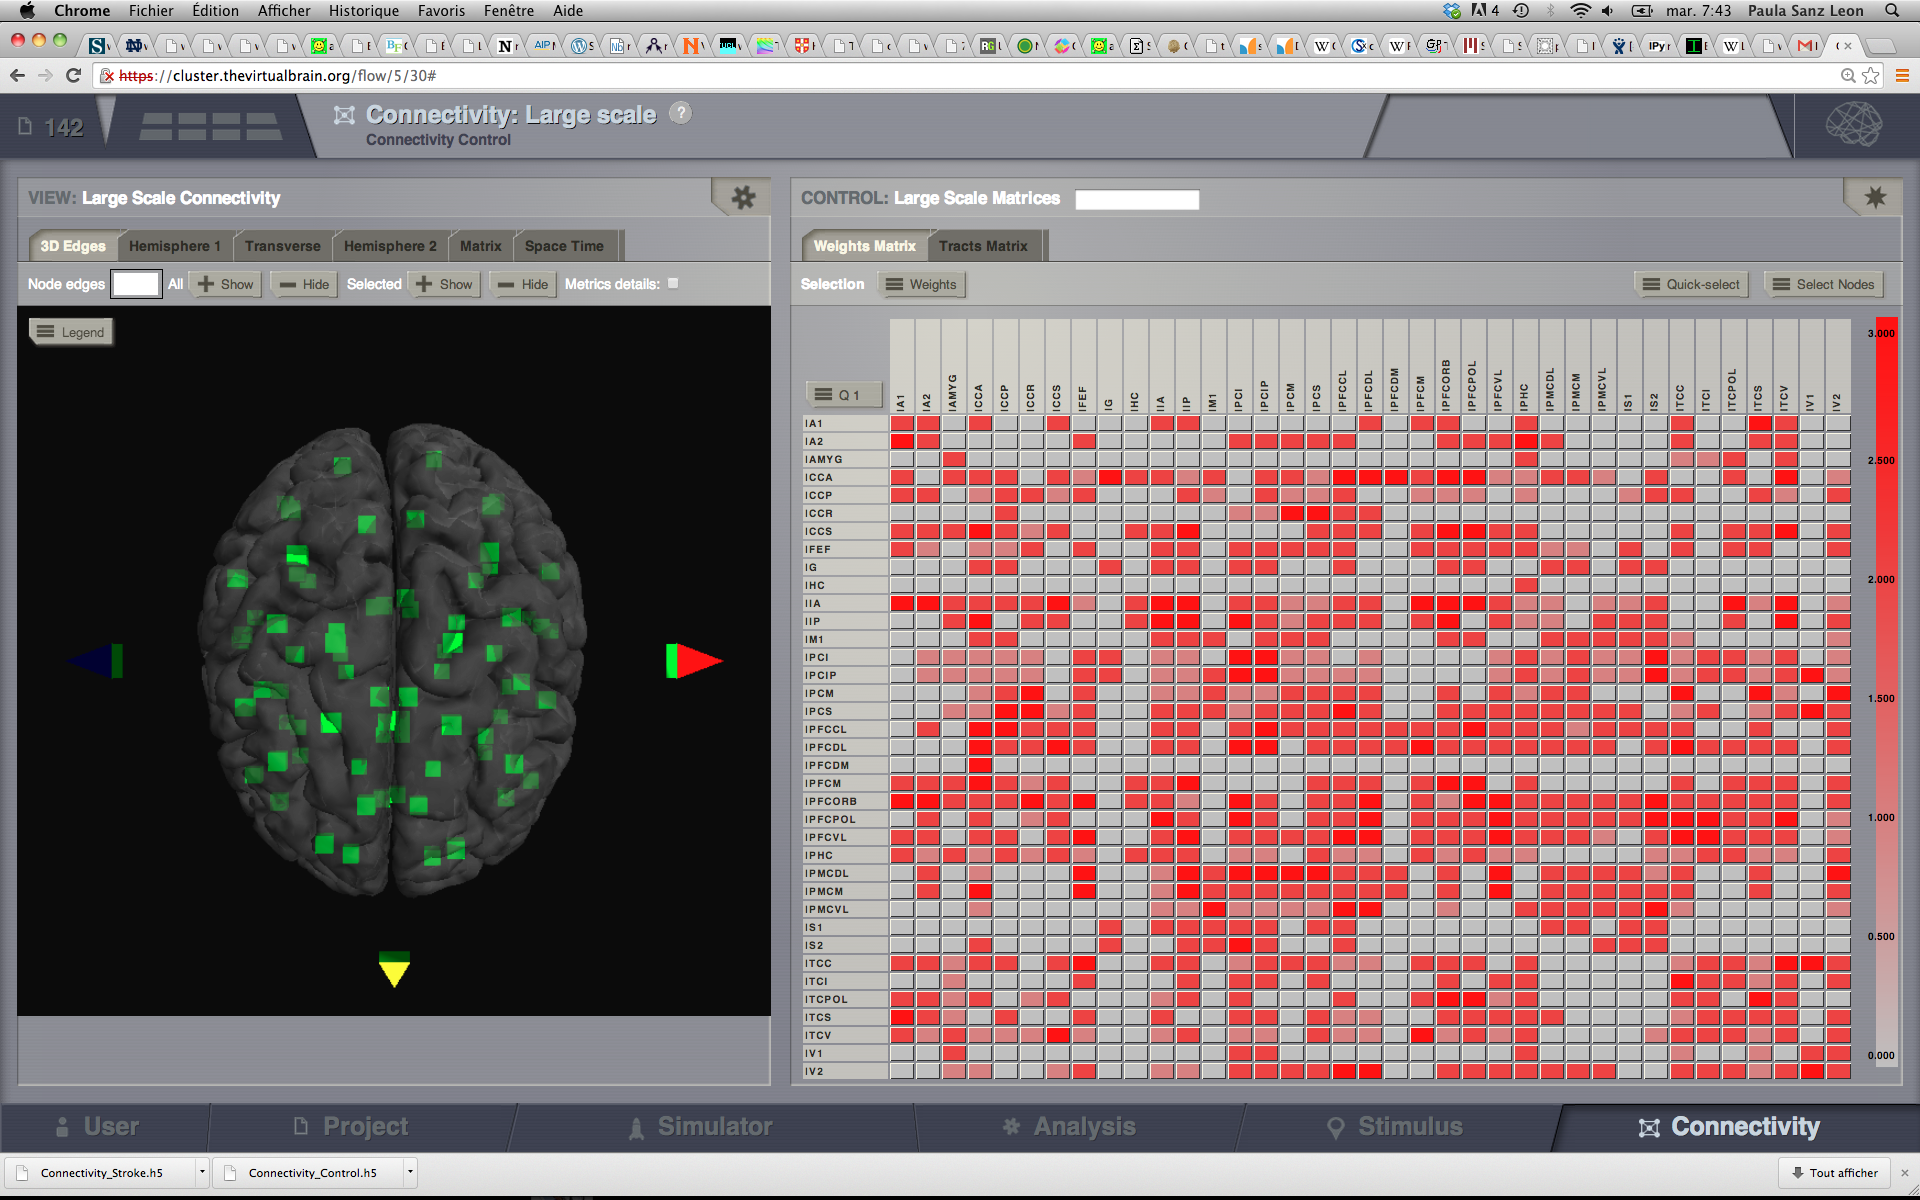
\includegraphics[width=\linewidth]{Handout_UI_ModellingStructuralLesions_ConnectivityArea}%
  \caption{Long-range connectivity editor}%
  \label{fig:fig}%
\end{figure}


\newpage
\subsection{Removing Interhemispheric Connections}\label{sec:steps}

\begin{marginfigure}%
  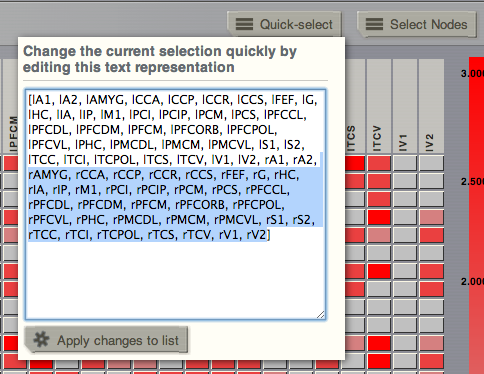
\includegraphics[width=\linewidth]{Handout_UI_ModellingStructuralLesions_QuickSelectRemoveNodes.png}%
  \caption{Remove the right nodes from the list.}%
  \label{fig:quickselect_removenodes}%
\end{marginfigure}%

\begin{marginfigure}%
  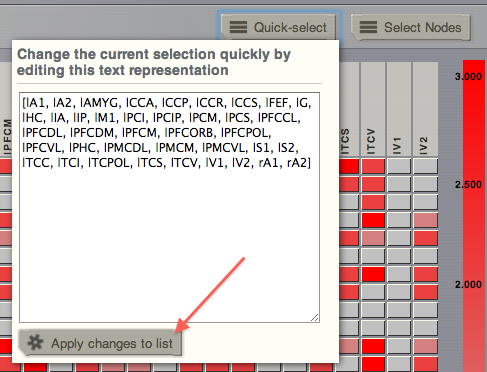
\includegraphics[width=\linewidth]{Handout_UI_ModellingStructuralLesions_QuickSelectApplyChanges.png}%
  \caption{Select only the left nodes and apply the changes.}%
  \label{fig:quickselect_applychanges}%
\end{marginfigure}%

\begin{marginfigure}%
  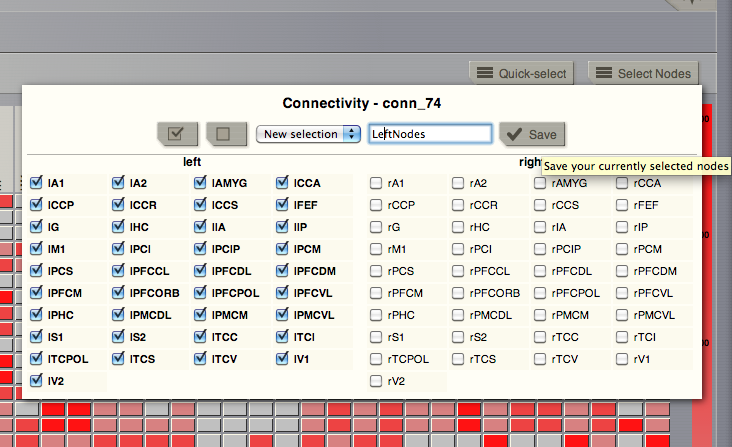
\includegraphics[width=\linewidth]{Handout_UI_ModellingStructuralLesions_SaveLeftNodes}%
  \caption{Save the left nodes selection.}%
  \label{fig:saveleftnodes}%
\end{marginfigure}%
\newthought{As a first step}, we will explore the TVB's default connectivity. Next, to model lesions, we will modify the connectivity, for
instance, by deleting edges or nodes. Here, as a working example we will remove the
interhemispheric connections. 

% (e.g., go through the different displays)

\begin{formal}
  \begin{enumerate}
  \item Go to the \textsc{Connectivity} area $\rightarrow$ \textsc{Large scale}.
  \item Select the the right nodes from the \underline{Quick Select} menu and delete them (Fig. \ref{fig:quickselect_removenodes}). Leave only the left nodes. (Fig. \ref{fig:quickselect_applychanges}). 
  \item Apply the changes. The active or selected nodes will appear in green on the left \underline{3D Edges}. 
  \item In the \underline{Select Nodes} menu, write a name for the new selection and save the selection for later use. (Fig. \ref{fig:saveleftnodes}). The connectivity editor will now be aware of two set of nodes: those in the selection (green) and those that have not been selected (white).
  \end{enumerate}
\end{formal}

\newpage


\begin{blah}
From the quadrant selector, move to the third quadrant (Q3). You can zoom in the display on the left and select a node next to the medial plane. Then, draw a node's ingoing and/or outgoing connections by selecting a node and then right-clicking on it. From the menu shown in Fig. \ref{fig:draw_connections} it is possible to make the edges visible and set their colour. 
\end{blah}
\begin{marginfigure}%
  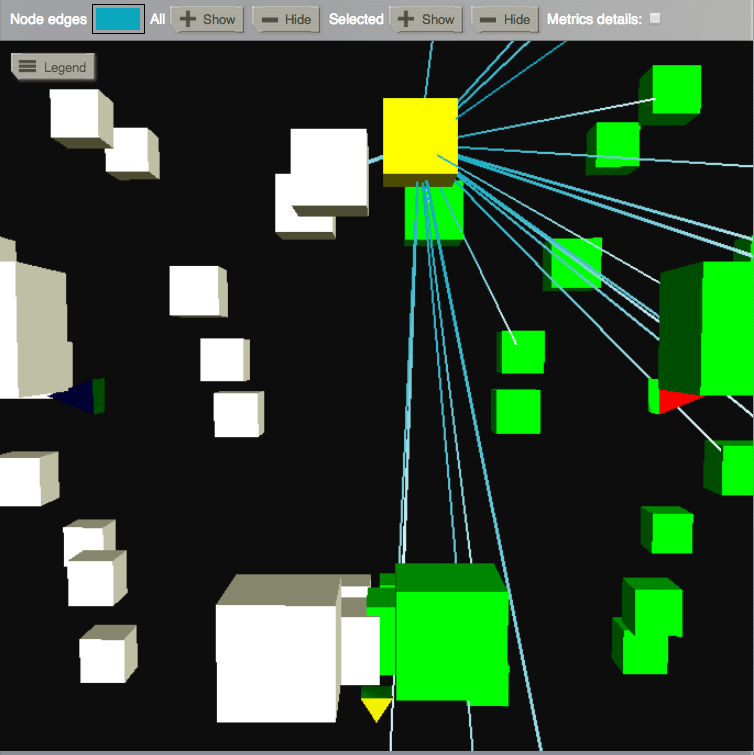
\includegraphics[width=\linewidth]{Handout_UI_ModellingStructuralLesions_DrawConnections}%
  \caption{Draw connections.}%
  \label{fig:draw_connections}%
\end{marginfigure}%

\noindent Now we'll proceed to perform operations on the edge values. 

\begin{formal}
  \begin{enumerate}[resume]
  \setcounter{enumi}{4}
  \item Click on the \underline{Weights}  menu and select the operation \textbf{Set(n)} for edges OUT-IN. Set the value to 0 and then apply the changes. 
  \item Select operation \textbf{Set(n)} for edges IN-OUT, set the value to 0 and then apply the changes. (Fig. \ref{fig:steps_05_06})
  \end{enumerate}
\end{formal}

\begin{marginfigure}
  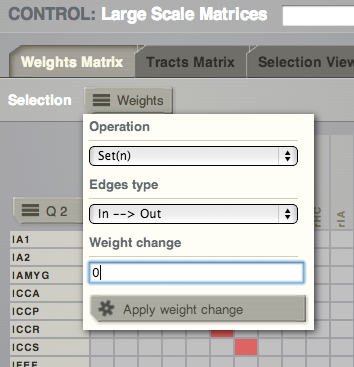
\includegraphics[width=\linewidth]{Handout_UI_ModellingStructuralLesions_EdgeOperations}%
  \caption{Set interhemispheric connections to 0}%
  \label{fig:steps_05_06}%
\end{marginfigure}


\begin{blah}
There are four category of edges depending on the nodes they connect:
\begin{itemize}
  \item Edges IN-IN. These edges connect pair of nodes in the \textit{selected set}. In this
  particular case you would modify the edges from the left hemisphere.
  \item Edges OUT-OUT. These edges connect pair of nodes in the \textit{unselected
  set}. In this case they would be the right intrahemispheric edges.
  \item Edges IN-OUT. These are the edges that connect nodes in the selected set
  (rows) to nodes in the unselected set (columns). In this case it refers to
  the edges in the second quadrant (Q2).
  \item Edges OUT-IN. These edges connect nodes in the unselected set (rows) to
  nodes in the selected set (columns). In this case it refers to the edges in the third
  quadrant (Q3).
\end{itemize}
\end{blah}


\begin{marginfigure}%
  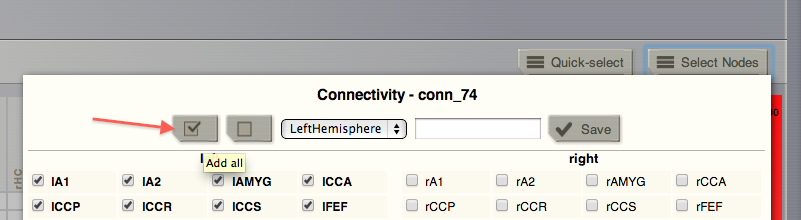
\includegraphics[width=\linewidth]{Handout_UI_ModellingStructuralLesions_SelectAllNodes}
    \caption{Select all nodes.}
  \label{fig:steps_selectall}
  \end{marginfigure}
  \begin{marginfigure}
 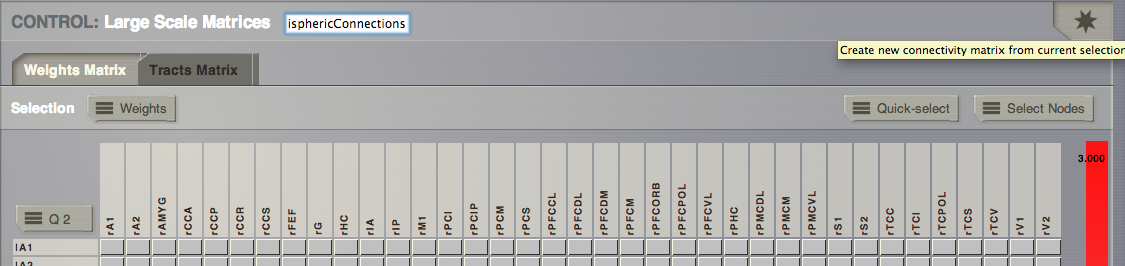
\includegraphics[width=\linewidth]{Handout_UI_ModellingStructuralLesions_SaveNewMatrix}
  \caption{Save a new connectivity.}
  \label{fig:steps_savenew}
\end{marginfigure}

\begin{formal}
  \begin{enumerate}[resume]
  \setcounter{enumi}{6}
    \item In the connectivity editor the interhemispheric connections are gone.
    Before you save the new connectivity matrix, make sure all the nodes are
included, otherwise TVB will assume you only want the nodes in the current
selection and will set the rest to zero. (Fig. \ref{fig:steps_selectall}).
   \item Give a name to the new connectivity and click on 
\includegraphics[width=0.08\textwidth]{butt_star_create.png} (Fig. \ref{fig:steps_savenew})
    \item The last action will take you back to the \textsc{Connectivity} $\rightarrow$ \textsc{Long-range connectivity}. From this page, load the new matrix. (Fig. \ref{fig:steps_07})
  \end{enumerate}
\end{formal}


\begin{figure}[h]
  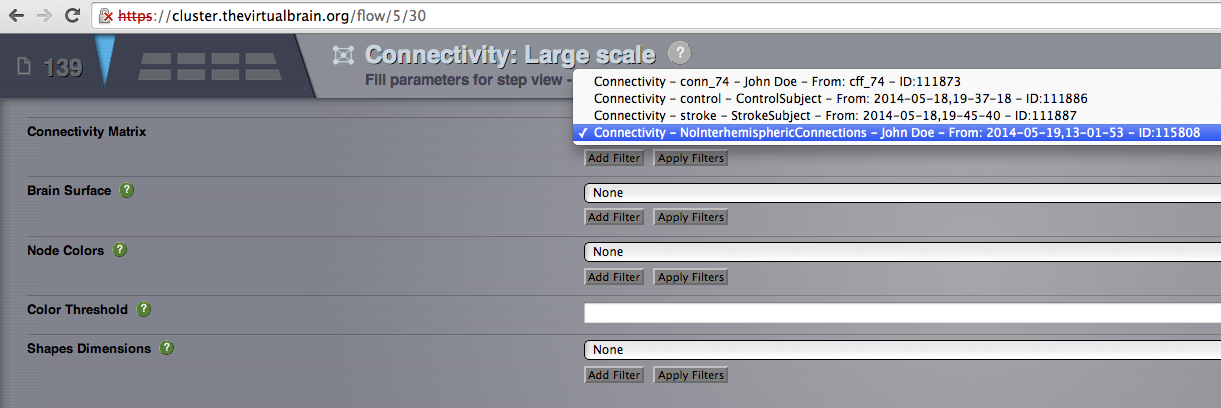
\includegraphics[width=\linewidth]{Handout_UI_ModellingStructuralLesions_LoadNewMatrix}%
  \caption{Load the newly created matrix.}%
  \label{fig:steps_07}%
\end{figure}

\subsection{Removing Nodes Based On Network Metrics}\label{sec:steps}

\newthought{Next, we'll use a criterion} based on graph-metrics to select which
nodes will be deleted. The metrics are computed using the BCT \sidenote{Brain Connectivity Toolbox} algorithms.  


\begin{marginfigure}
  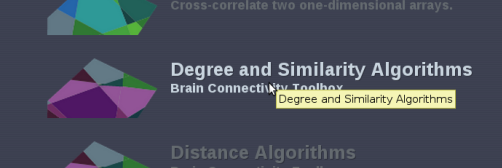
\includegraphics[width=\linewidth]{Handout_UI_ModellingStructuralLesions_Analysis}%
  \caption{Compute network metrics}%
  \label{fig:degree_similarity}%
\end{marginfigure}

%%%%%%%%%%%%%%%%%%%%%%%%%% STEPS %%%%%%%%%%%%%%%%%%%%%%%%%%%%%%%%%%%%%
\begin{formal}
  \begin{enumerate}[resume]
  \setcounter{enumi}{9}
  \item Go to \textsc{Analysis} $\rightarrow$ \textsc{Degree and similarity algorithms}.  (Fig. \ref{fig:degree_similarity}).
  \item Select the metric \textbf{Degree} and \textbf{TVB's default connectivity matrix} as input. Click on \underline{Launch}.
  \item Repeat the previous step for the following metrics: \textbf{Indegree and Outdegree, Strength, Instrength and Outstrength}.
  \end{enumerate}
\end{formal}
%%%%%%%%%%%%%%%%%%%%%%%%%%%%%%%%%%%%%%%%%%%%%%%%%%%%%%%%%%%%%%%%%%%%%

\begin{marginfigure}
  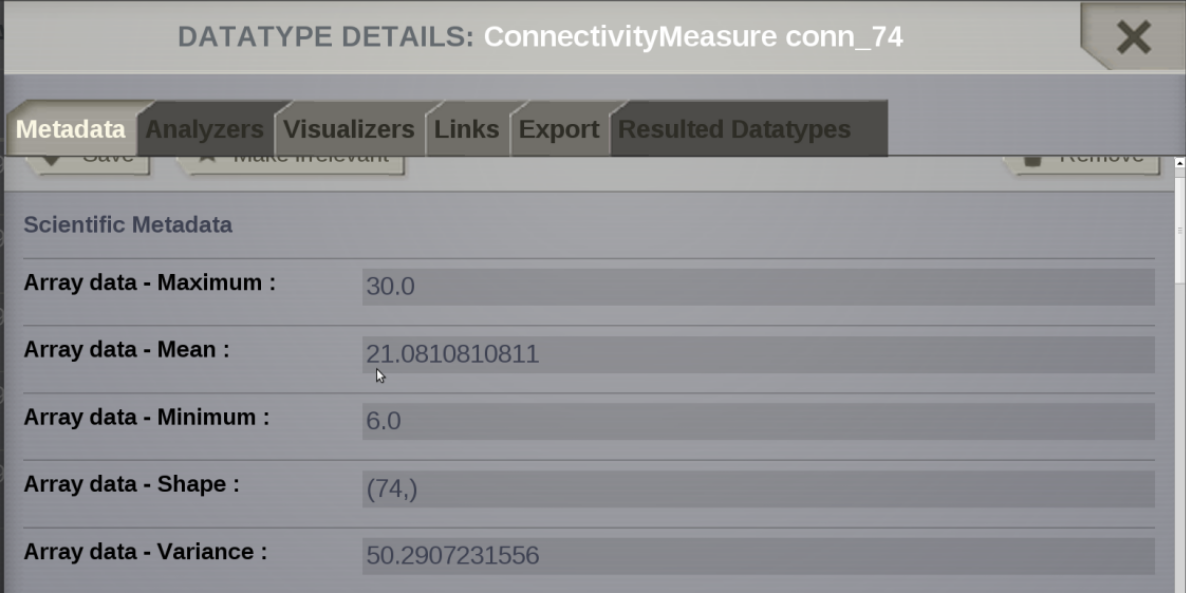
\includegraphics[width=\linewidth]{Handout_UI_ModellingStructuralLesions_AnalysisResult}%
  \caption{Descriptive summary}%
  \label{fig:step_02}%
\end{marginfigure}

\begin{formal}
  \begin{enumerate}[resume]
  \setcounter{enumi}{12}
  \item Go back to \textsc{projects} $\rightarrow$ \textsc{Operations dashboard}.
  \item Click on 
\includegraphics[width=0.042\linewidth]{nodeConnectivityMeasure}. On
  the overlay window you can already see a summary of the basic descriptive
  statistics (Fig.~\ref{fig:step_02}).
  \item You can display the results as a histogram by launching the \underline{Connectivity Measure Visualizer}. However, here we'll launch the \underline{Topographic Viewer}. This 2D layout of the
head gives an idea of the network topology based on the node-wise
metrics. 
  \end{enumerate}
\end{formal}


%%%%%%%%%%%%%%%%%%%%%%%%%% STEPS %%%%%%%%%%%%%%%%%%%%%%%%%%%%%%%%%%%%%
\newpage

\begin{marginfigure}
  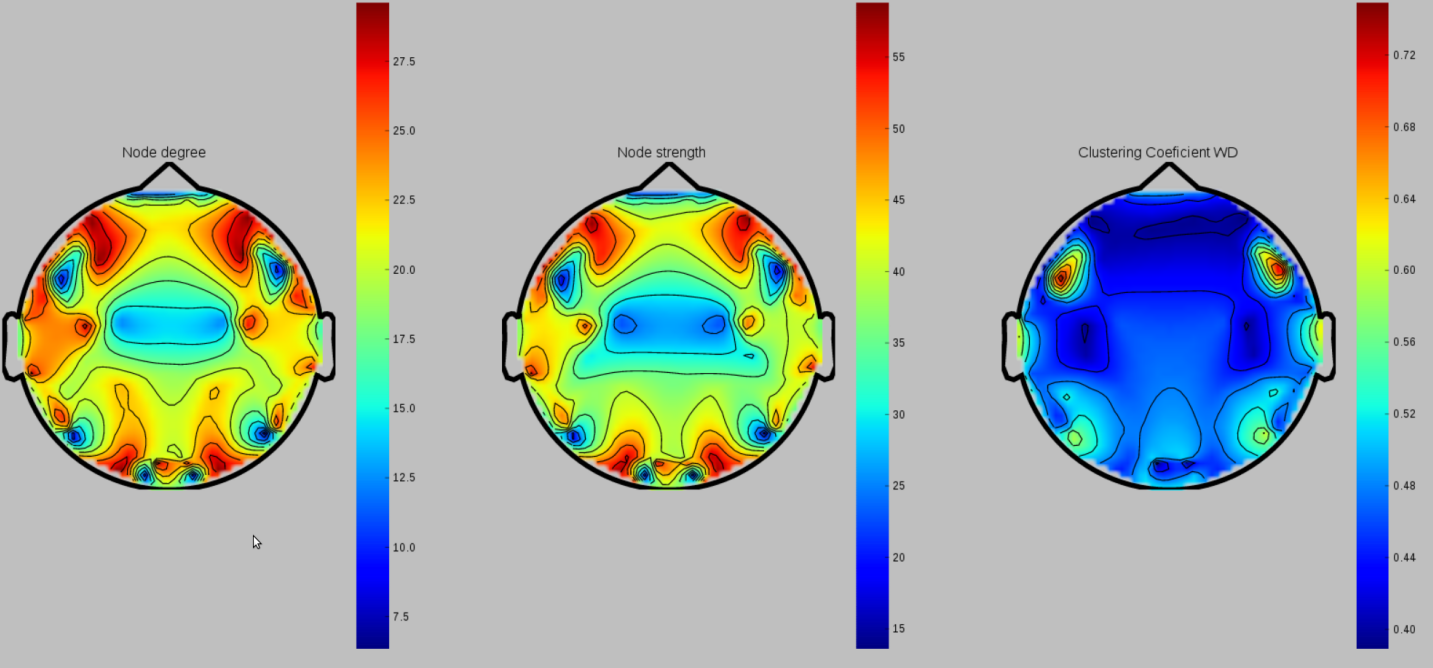
\includegraphics[width=\linewidth]{Handout_UI_ModellingStructuralLesions_AnalysisResultCompare}%
  \caption{View and compare network metrics}%
  \label{fig:step_05b}%
\end{marginfigure}
\begin{marginfigure}
  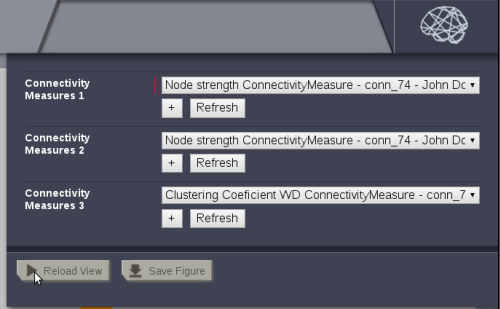
\includegraphics[width=\linewidth]{Handout_UI_ModellingStructuralLesions_AnalysisView}%
  \caption{Select additional metrics}%
  \label{fig:step_05}%
\end{marginfigure}


\noindent Since other network measures were previously computed so we can also have a look at them. 
\begin{formal}
  \begin{enumerate}[resume] %% doesnt work with the formal enviornment :/
  \setcounter{enumi}{15}
  \item In this visualizer, it is possible to view and compare up to three metrics (Fig. ~\ref{fig:step_05b}). From the menu 
\includegraphics[width=0.08\textwidth]{butt_brain_menu} on the top right select \textbf{strength} and \textbf{clustering coefficient}. Click on \underline{Update Visualizer}. (See Fig. ~\ref{fig:step_05})
  \end{enumerate}
\end{formal}
%%%%%%%%%%%%%%%%%%%%%%%%%%%%%%%%%%%%%%%%%%%%%%%%%%%%%%%%%%%%%%%%%%%%%

\begin{formal}
  \begin{enumerate}[resume] %% doesnt work with the formal enviornment :/
  \setcounter{enumi}{16}
  \item Go back to the \textsc{Connectivity} $\rightarrow$ \textsc{Large scale connectivity} area. 
  \item  In the field \underline{Node colors} select
the node-wise \textbf{Instrength, ID: 116005} .
\item Set a \underline{Color threshold} of \textbf{56}. Launch the connectivity editor.
  \item Go to the \underline{Transverse visualizer}, which displays a spring-like layout of the network graph (top view). Click on \underline{Show all} to apply the threshold previously set. Fig. \ref{fig:step_12}
  \end{enumerate}
\end{formal}

\begin{marginfigure}
  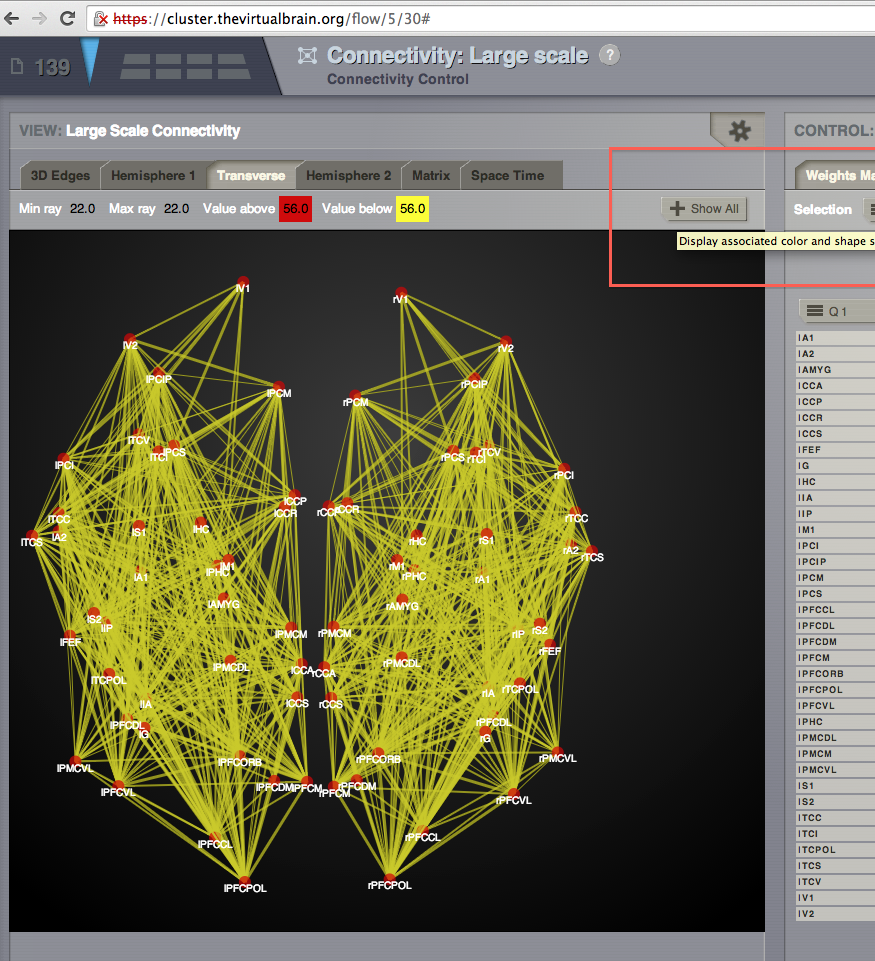
\includegraphics[width=0.9\linewidth]{Handout_UI_ModellingStructuralLesions_ShowColourNodes}%
  \caption{Show node colours.}%
  \label{fig:step_12}%
\end{marginfigure}

\begin{formal}
  \begin{enumerate}[resume] %% doesnt work with the formal enviornment :/
  \setcounter{enumi}{20}
\item To completely remove the nodes, from \underline{Quick select} we create a selection excluding these high in-strength nodes (Fig. \ref{fig:step_subnetwork}) and directly save the new matrix. 
%or,
%\item create a small selection with the high in-strength nodes (Fig. \ref{fig:step_subnetwork}) and use \underline{Edge operations} to  set the IN-IN, IN-OUT and OUT-IN edges to zero. Here, we did the latter.
\item From 
\includegraphics[width=0.08\textwidth]{butt_brain_menu} 
 you can change the measure used to colour the nodes as well as the threshold  (Fig. \ref{fig:step_change_threshold}). Repeat the necessary steps using \textbf{Degree}. 

  \end{enumerate}
\end{formal}

\begin{marginfigure}
  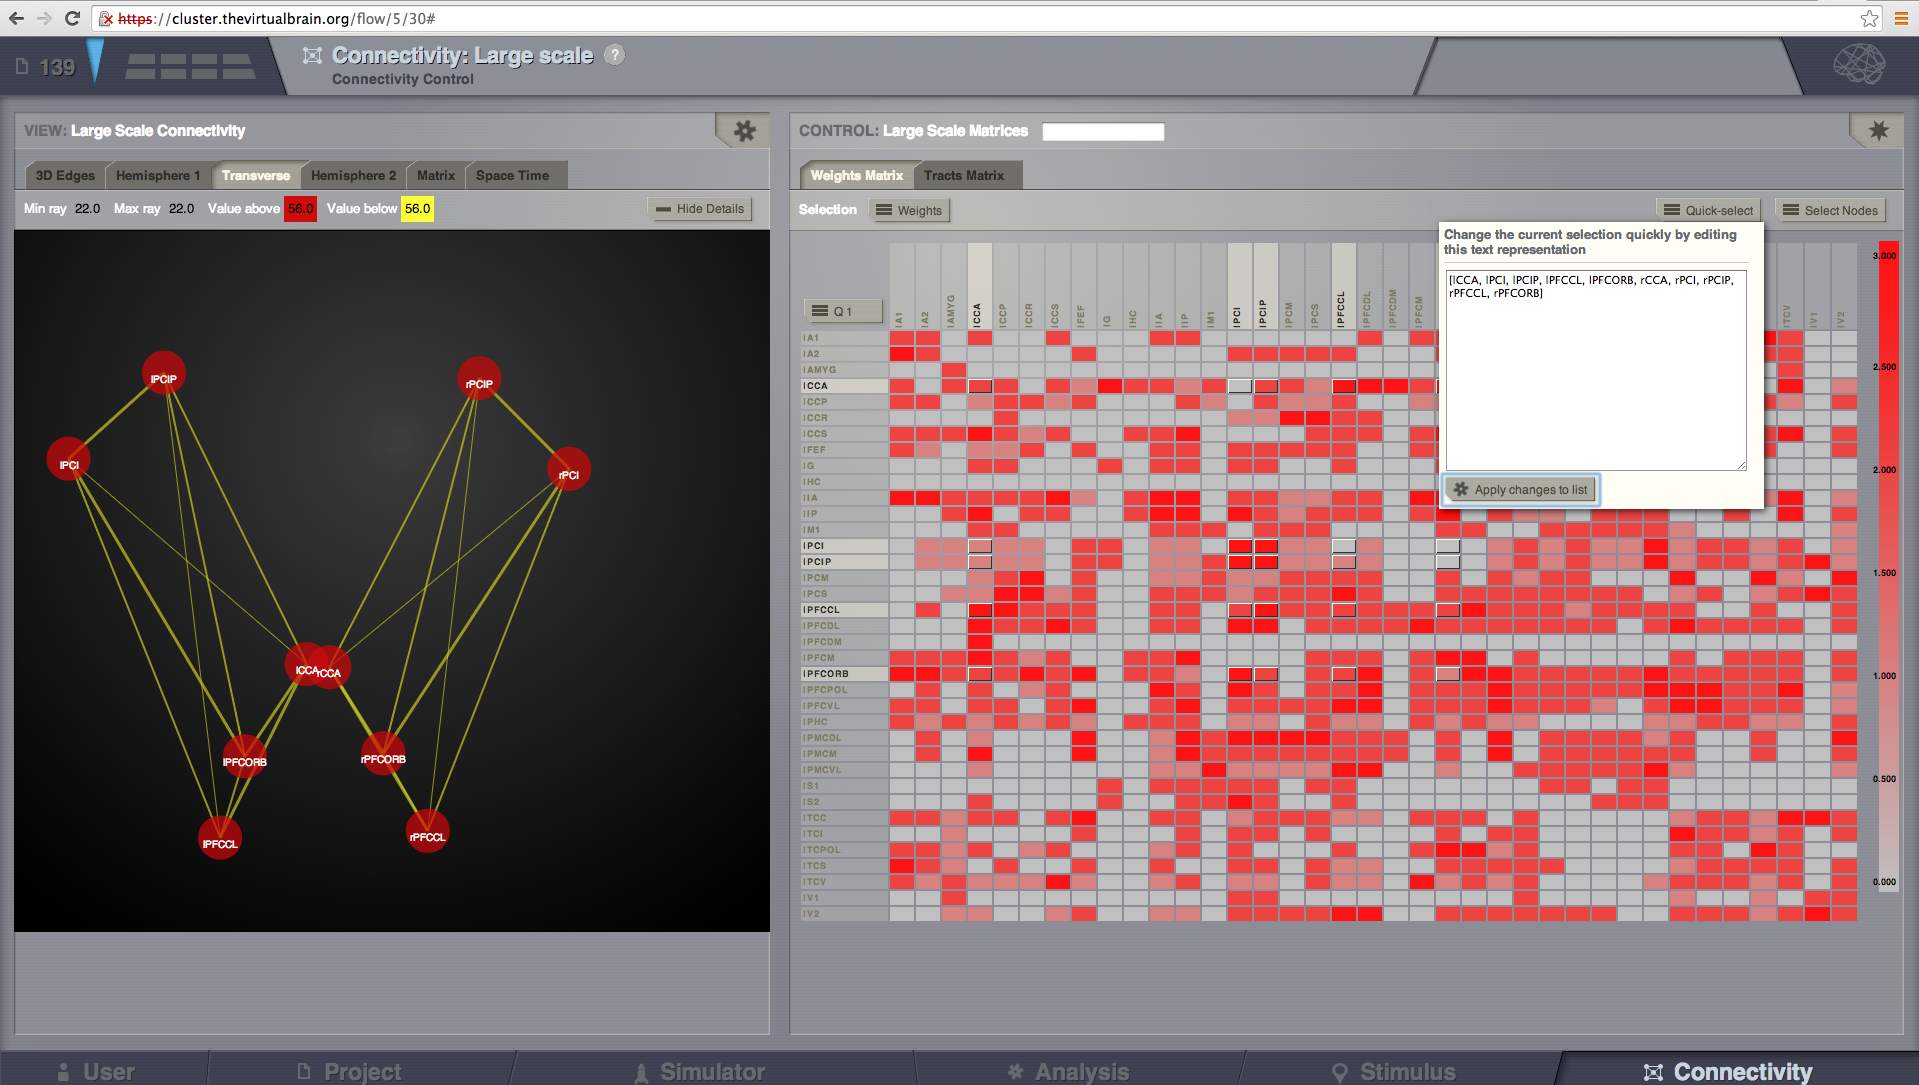
\includegraphics[width=0.9\linewidth]{Handout_UI_ModellingStructuralLesions_SelectSubnetwork}%
  \caption{Select subnetwork with the highest in-strength nodes.}%
  \label{fig:step_subnetwork}%
\end{marginfigure}
\vspace{1.1cm}
\begin{figure}[h]
  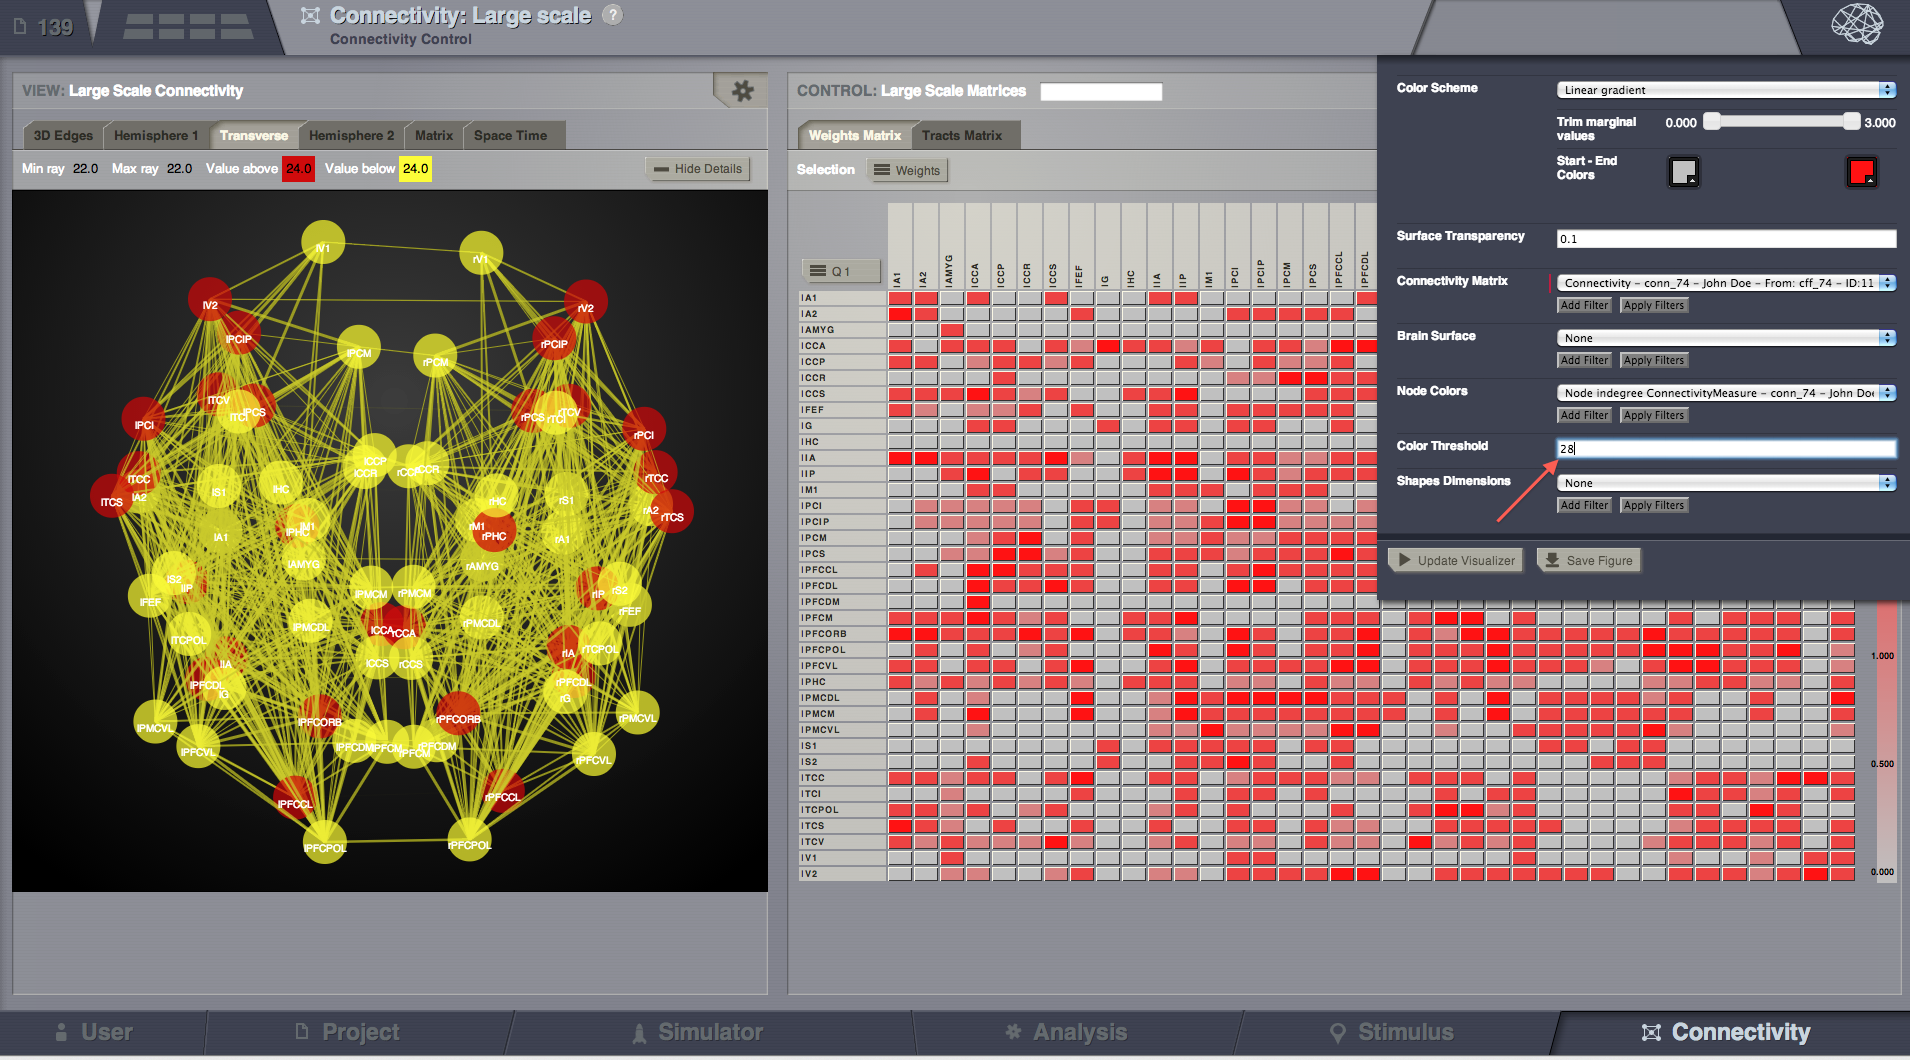
\includegraphics[width=0.9\linewidth]{Handout_UI_ModellingStructuralLesions_ChangeNodeColourThreshold}%
  \caption{Change the metric and threshold.}%
  \label{fig:step_change_threshold}%
\end{figure}
\newpage

\subsection{The Effect Of The Structural Connectivity On The Global Stability Map}
 \begin{marginfigure}%
  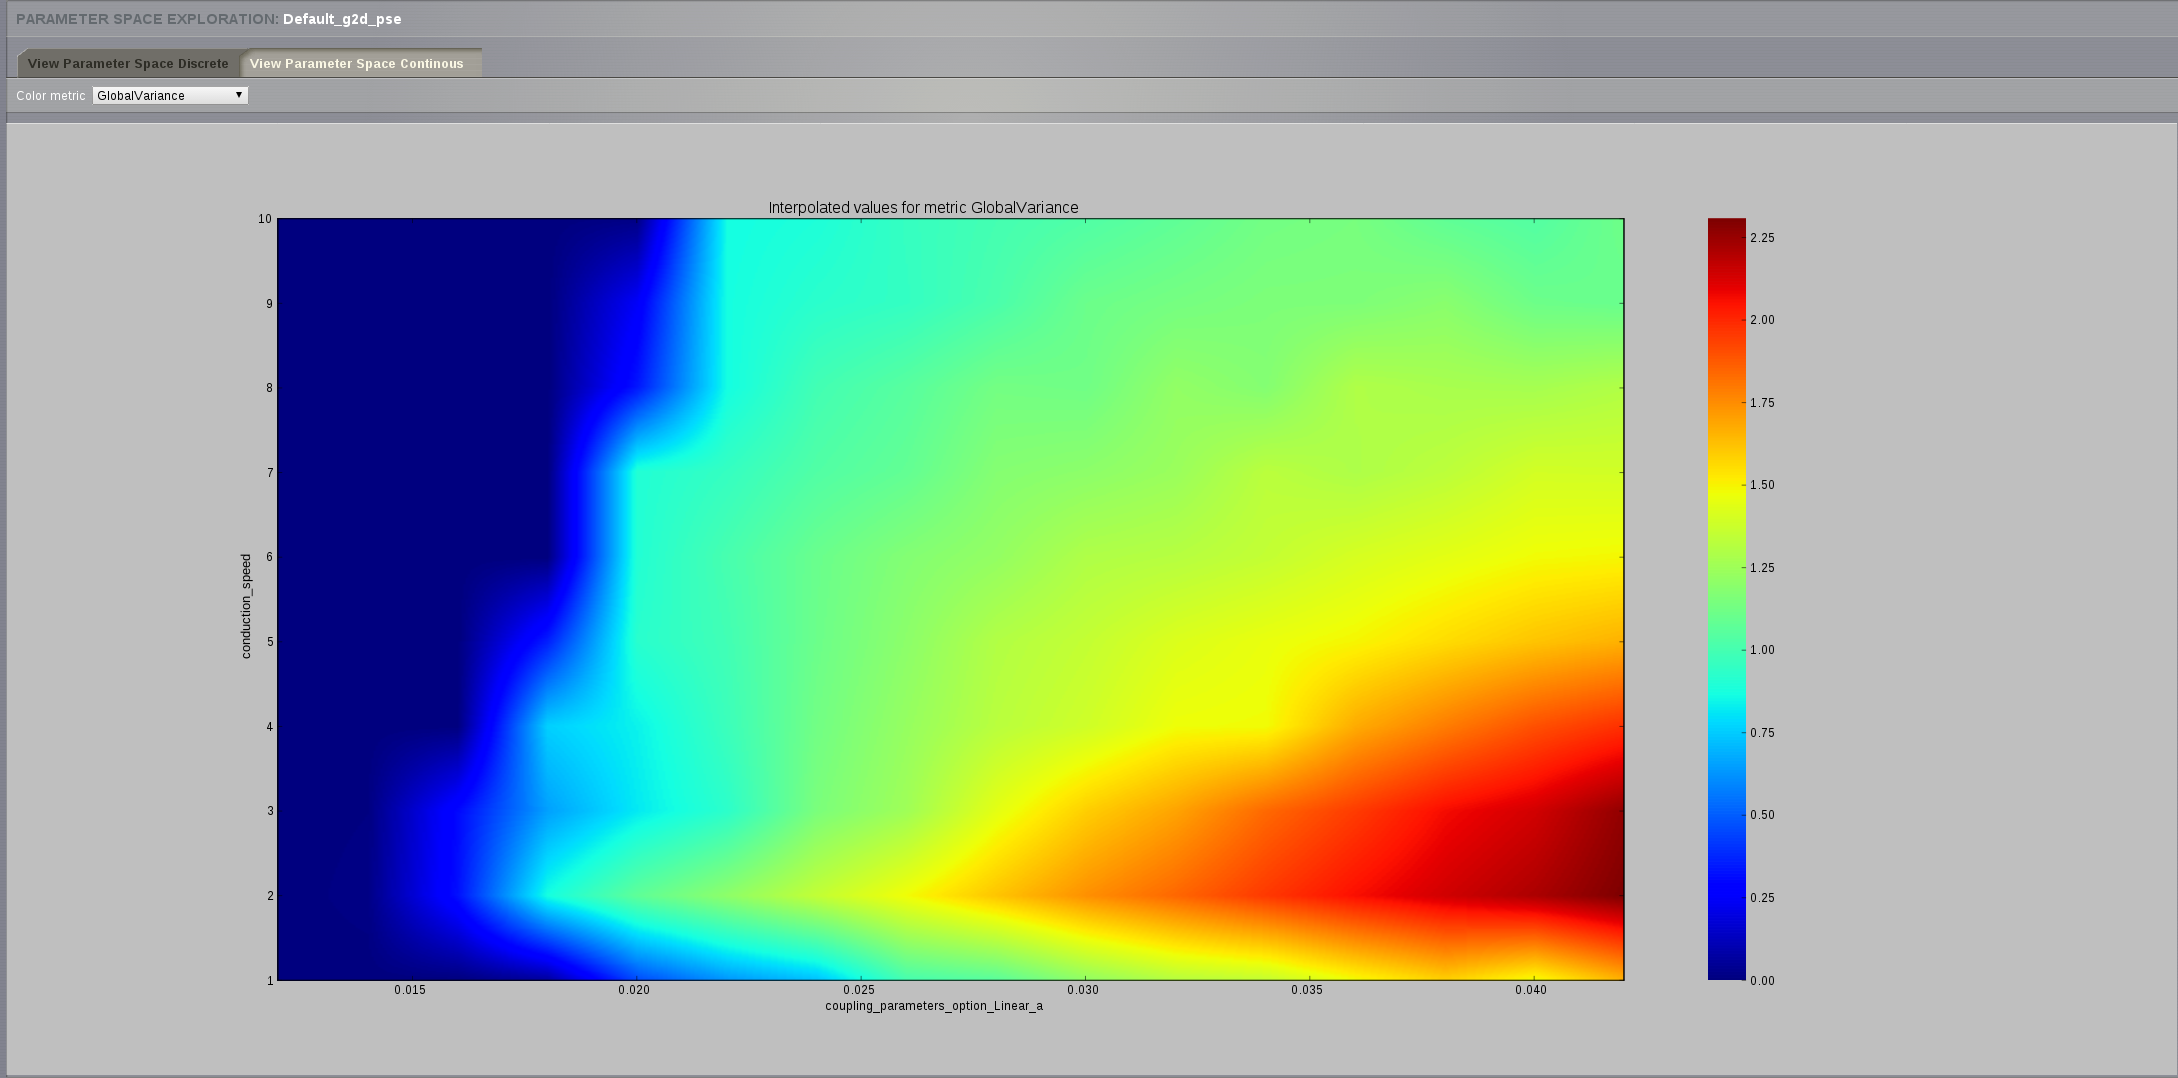
\includegraphics[width=\linewidth]{Handout_UI_ModellingStructuralLesions_DefaultPSE}
    \caption{Global variance map from $\circ$  \textit{Default\_g2d\_pse}}
  \label{fig:default_pse}
  \end{marginfigure}
 \begin{marginfigure}%
  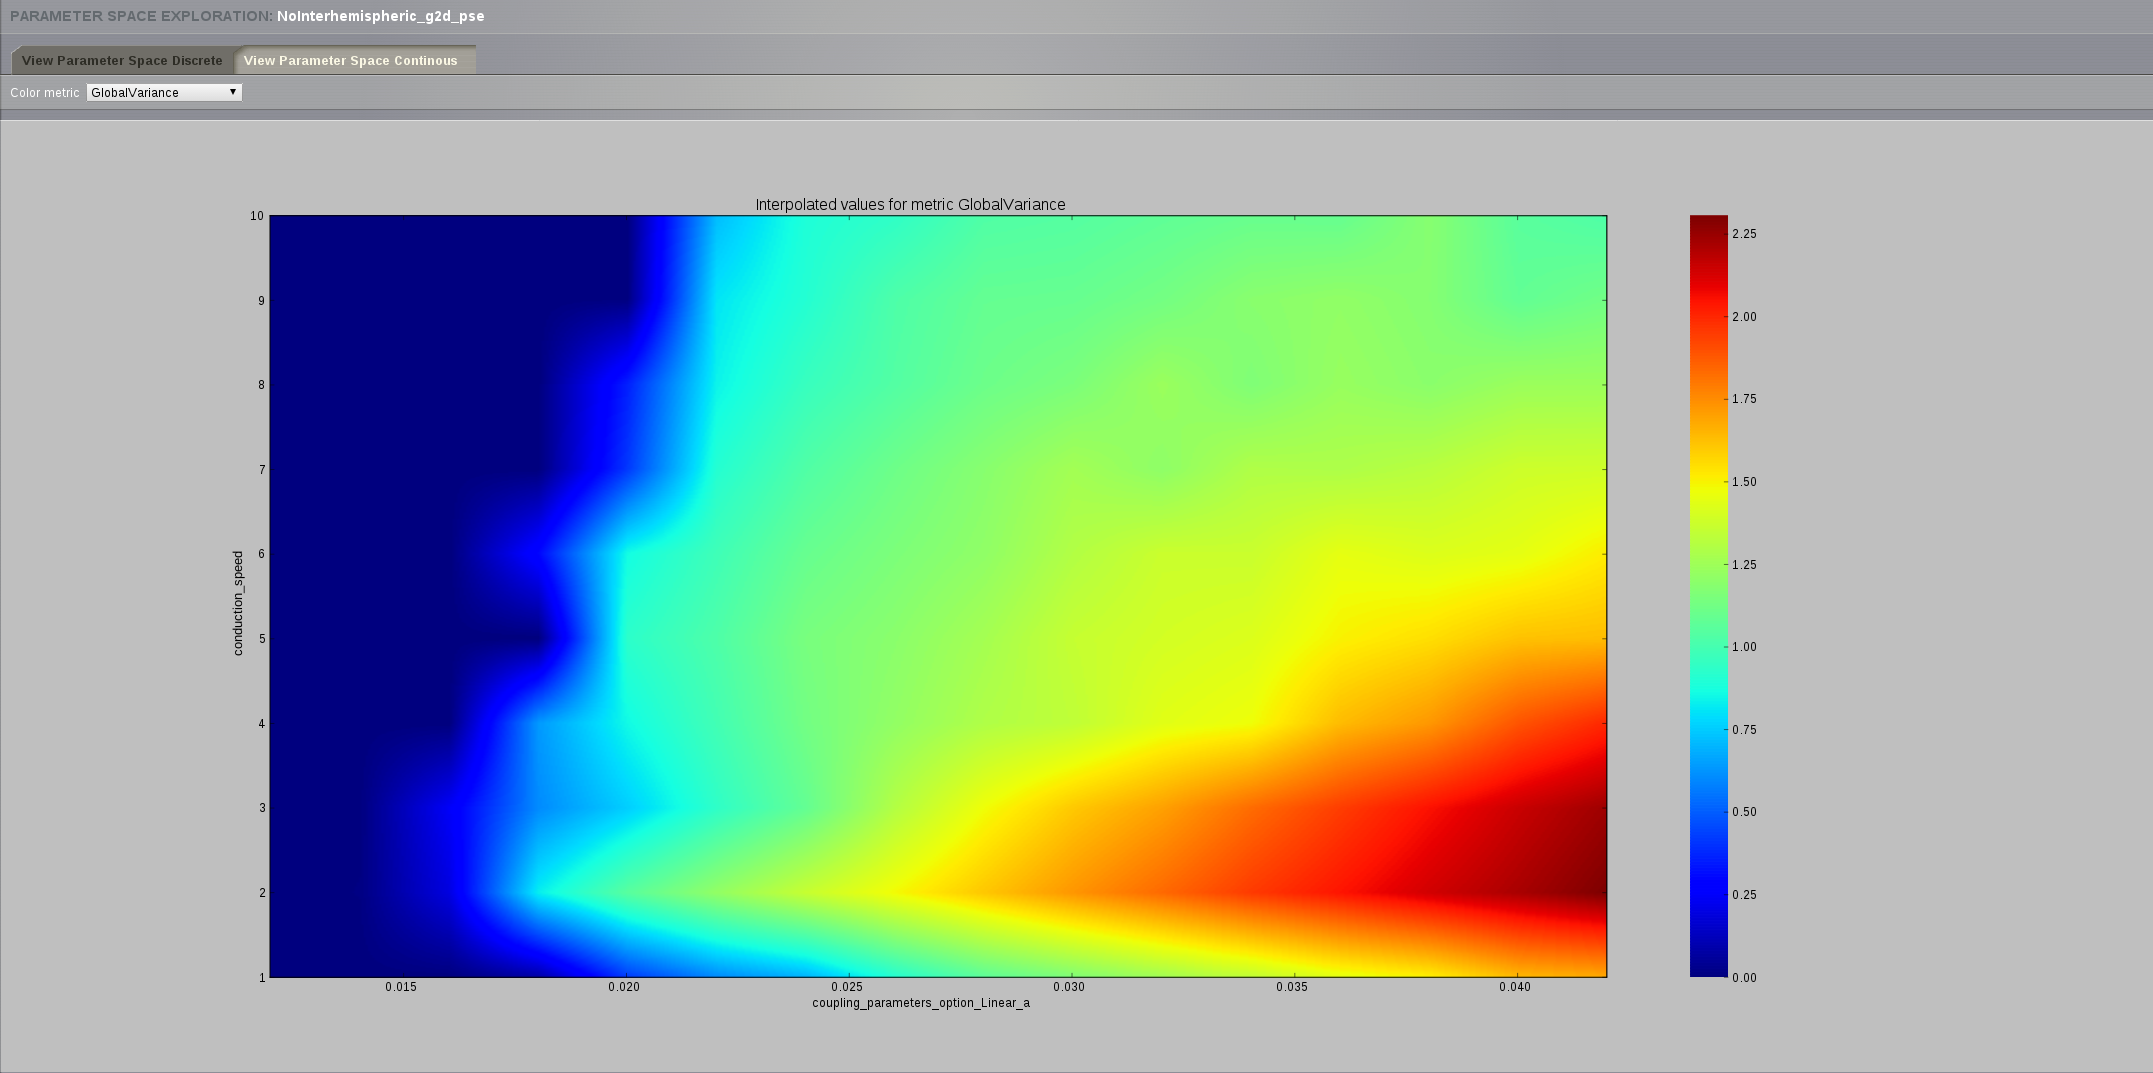
\includegraphics[width=\linewidth]{Handout_UI_ModellingStructuralLesions_NoInterHemisphericPSE}
    \caption{Global variance map from $\circ$  \textit{NoInterhemispheric\_g2d\_pse}}
  \label{fig:nointer_pse}
  \end{marginfigure}
 \begin{marginfigure}%
  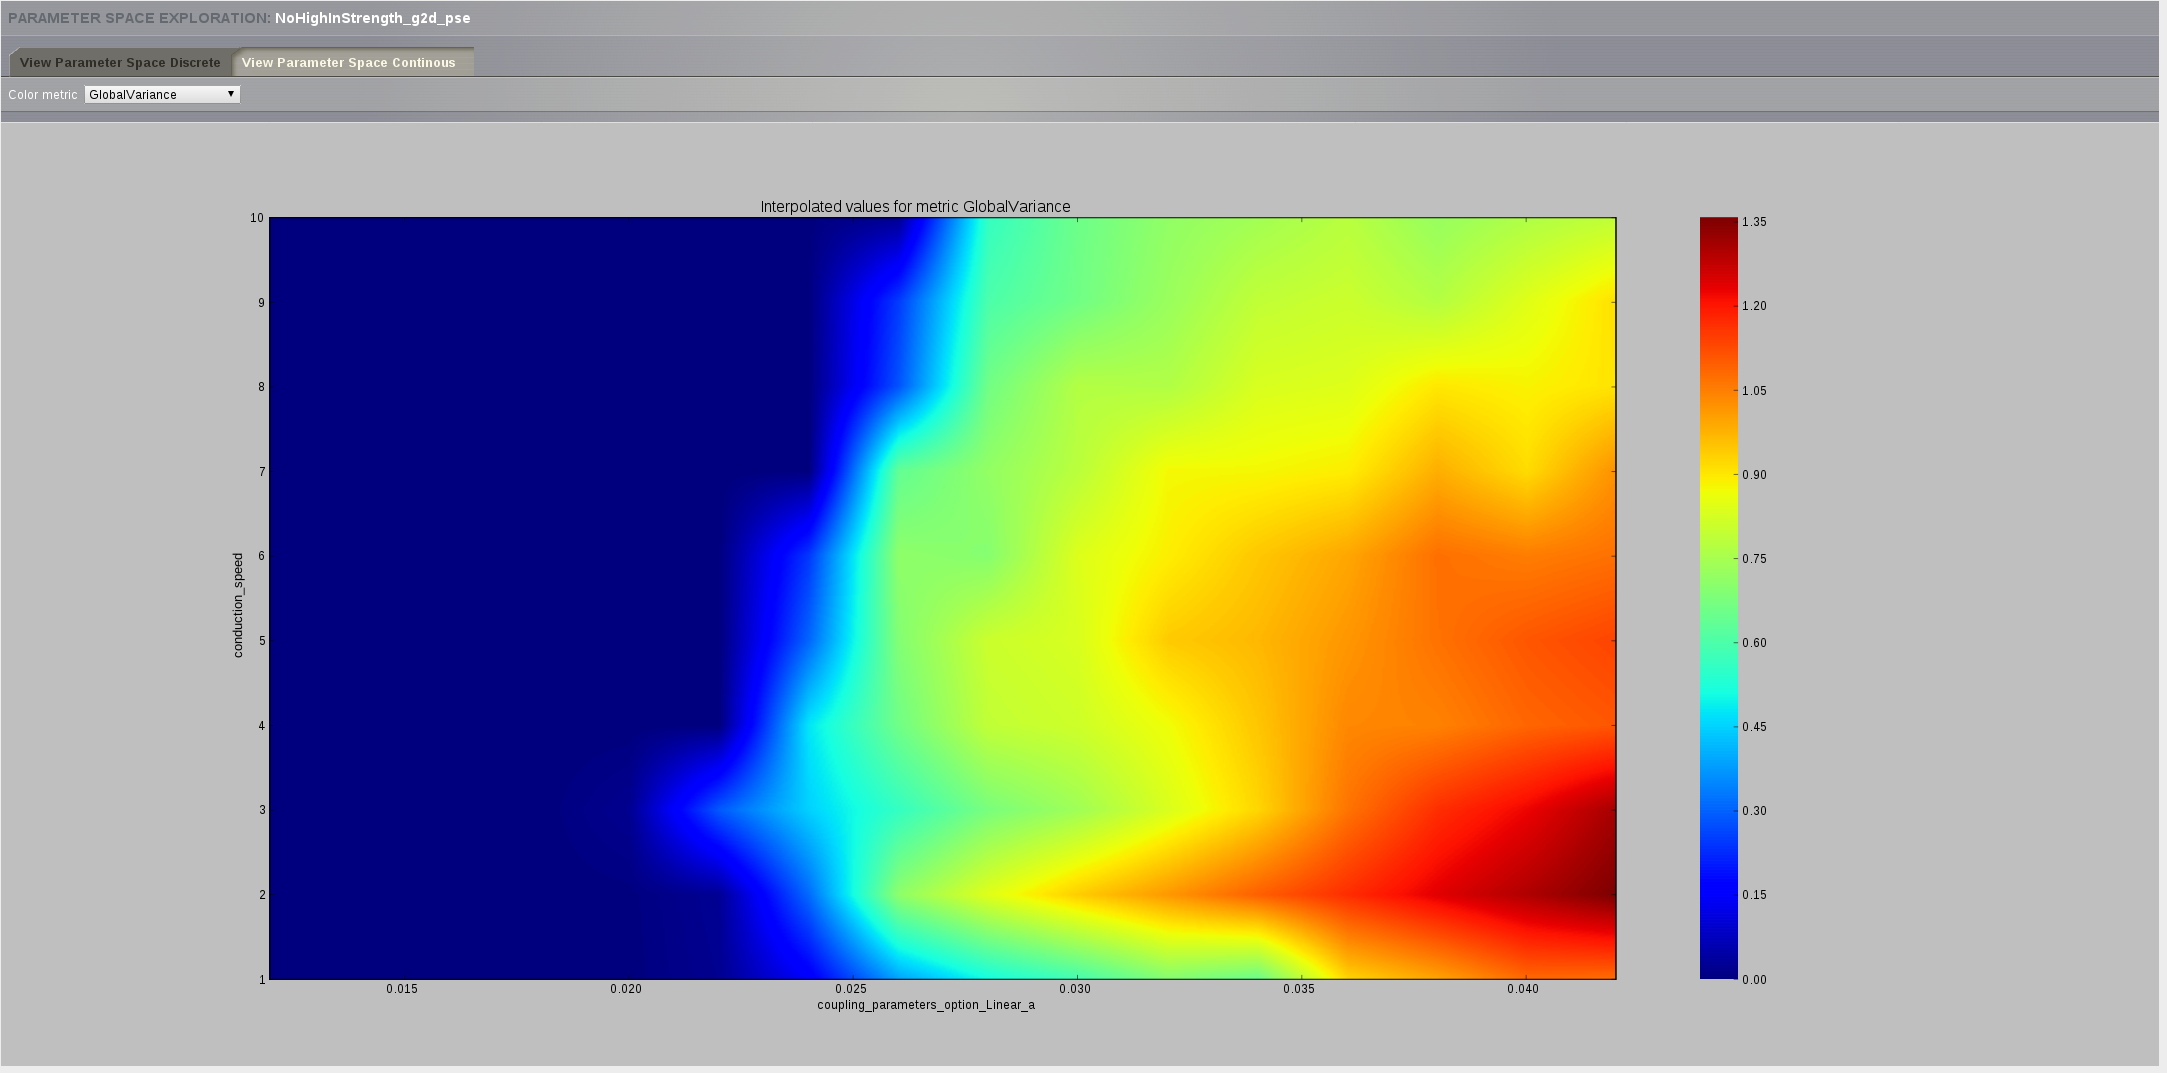
\includegraphics[width=\linewidth]{Handout_UI_ModellingStructuralLesions_NoHighInStrengthPSE}
    \caption{Global variance map from $\circ$  \textit{NoHighInStrength\_g2d\_pse} }
  \label{fig:nostrength_pse}
  \end{marginfigure}
 \begin{marginfigure}%
  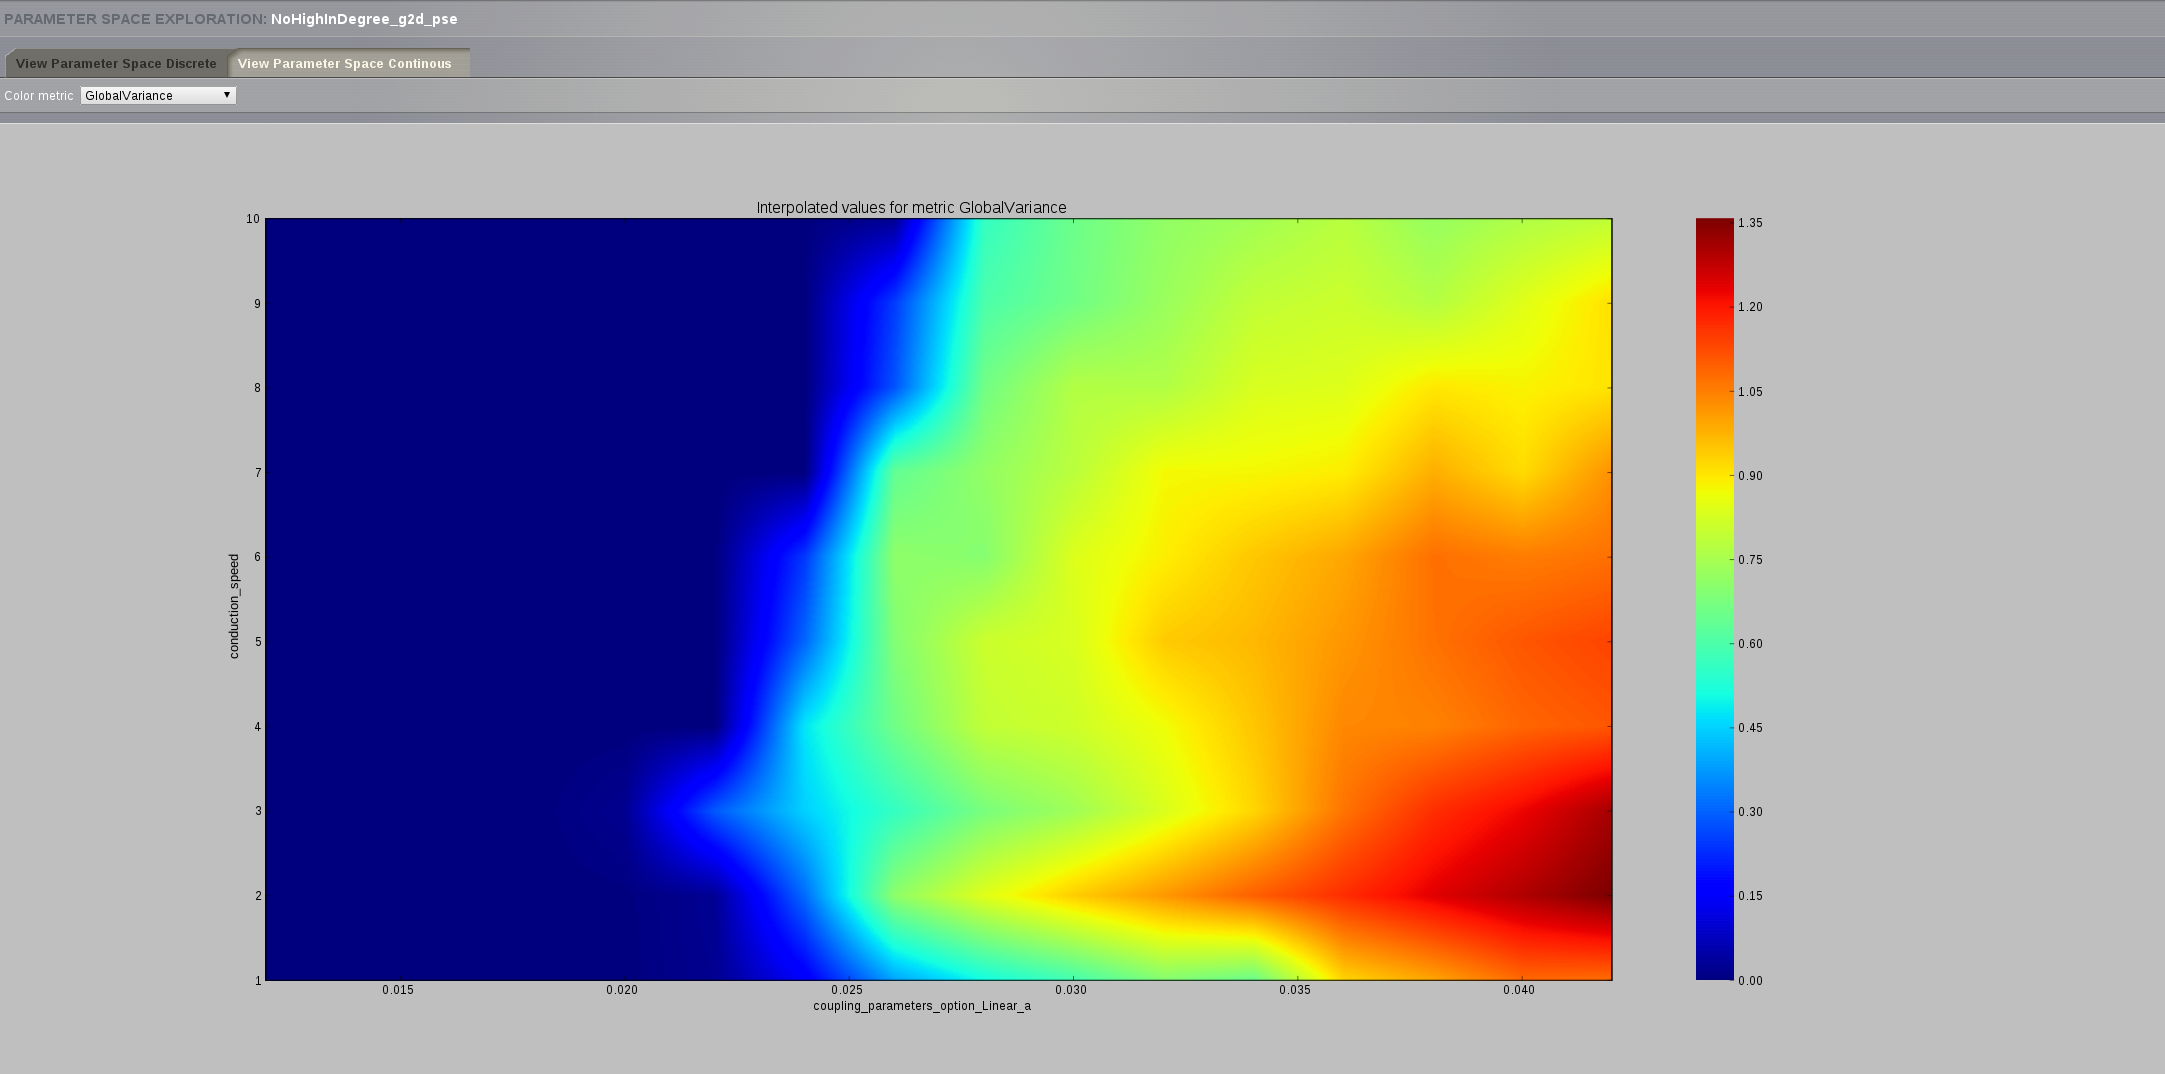
\includegraphics[width=\linewidth]{Handout_UI_ModellingStructuralLesions_NoHighInDegreePSE}
    \caption{Global variance map from $\circ$  \textit{NoHighInDegree\_g2d\_pse}}
  \label{fig:nodegree_pse}
  \end{marginfigure}
  
\begin{simulation}
\begin{enumerate}
\item Go to \textsc{simulator}. Copy the simulation \textit{Control\_g2d\_pse}.  Launch a \underline{Parameter Space Exploration} (PSE) using \textbf{TVB's default connectivity}.
\item Repeat the previous step but using the following matrices \textbf{NoInterhemispheric, NoHighInStrength} and \textbf{NoHighInDegree}.
These are simulations $\circ$  \textit{Default\_g2d\_pse}, $\circ$ \textit{NoInterhemispheric\_g2d\_pse}, $\circ$ \textit{NoHighInStrength\_g2d\_pse} and $\circ$ \textit{NoHighInDegree\_g2d\_pse}. Their respective PSE maps are displayed in Figs. \ref{fig:default_pse}, \ref{fig:nointer_pse}, \ref{fig:nostrength_pse} and \ref{fig:nodegree_pse}.
\end{enumerate}
\end{simulation}



\subsection{Region-based Simulations Of A Control And Stroke Connectome}

\newthought{We will now} to evaluate the difference between the activity generated by both control and stroke connectivity matrices. We'd like to see how the structural differences alter the stability plane of our system. 


\begin{simulation}
  \begin{enumerate}
  \item Go to the \textsc{simulator} area. 
  \item Select the \textbf{control connectivity, ID: 111886}. We proceed to launch a PSE using the same model and simulation parameters as found in Table 2 of the first session. This is simulation \textit{Control\_g2d\_pse}.
  \item Copy the previous simulation and launch a second PSE where, but this time use the \textbf{stroke connectivity, ID:111887}. The results are in simulation \textit{Stroke\_g2d\_pse}.
  \item Select a point in the resulting \underline{Parameter Space Discrete} map, for instance the one with \underline{conduction speed} equal to \textbf{\unitfrac[7]{mm}{ms}} and \underline{global coupling strength} \textbf{a}$\mathbf{=}$\textbf{\unit[0.008][au]}. Tag the time-series (e.g \underline{Datatype Tag 3}: \textbf{ThisPoint}). 
  
 \item Repeat the previous step for the same point in \textit{Control\_g2d\_pse}.
 
  \item Then, using the parameters from the previously tagged points, launch two \textbf{\unit[60]{s}} long simulations. 
  \item  Use the \textbf{BOLD monitor} and the \textbf{Mixture of Gammas} \underline{HRF kernel} with its default parameters. The \underline{sampling period} of the monitor is \textbf{\unit[2000]{ms}}. 
\end{enumerate}
\end{simulation} 

These two simulations are not included in this project, but you will need them if you want to reproduce the simulations  described below. 


\begin{simulation}
\begin{enumerate}[resume]
\setcounter{enumi}{6}
  \item Using the branching mechanism, launch \textbf{\unit[4]{min}} simulations from the two previous ones. 
  \end{enumerate}
\end{simulation}

These are \textit{Control\_g2d\_init\_bold\_branch1} and \textit{Stroke\_g2d\_init\_bold\_branch1}.

 
 \begin{marginfigure}%
  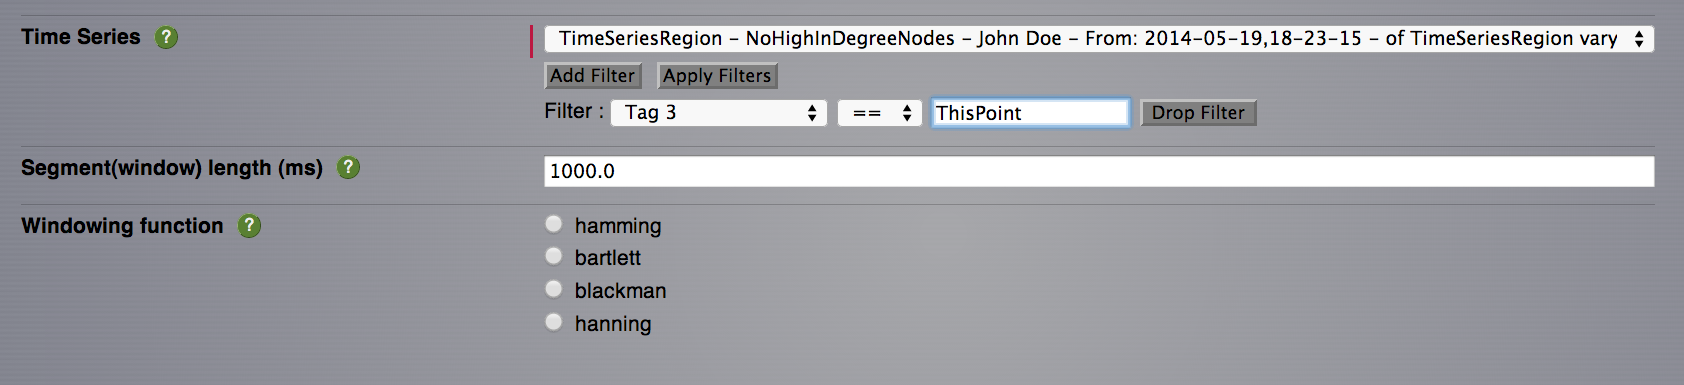
\includegraphics[width=0.82\linewidth]{Handout_UI_ModellingStructuralLesions_FourierAddFilter}
    \caption{Add and apply a filter.}
  \label{fig:fourier_addfilter}
  \end{marginfigure}
 \begin{formal}
  \begin{enumerate}
  \item Go to \textsc{Analysis} $\rightarrow$\textsc{Fourier spectral analysis}. 
  \item Add and apply a filter to find the time-series tagged with \textit{ThisPoint}. (Fig. \ref{fig:fourier_addfilter}). Select \textbf{All}.
  \item Select a \textbf{Hamming} \underline{window} with a length of \textbf{\unit[500]{ms}}.  Launch the analyzer. (See Fig. \ref{fig:steps_sim_03}).
  \item Go to \textsc{Projects}$\rightarrow$\textsc{Operation dashboard} and have a look at the spectra of the time-series.
 \end{enumerate}
\end{formal}

\subsection{Region-based Simulations Of A Control And Stroke Connectome Using A Higher-dimensional Model}

\begin{marginfigure}%
  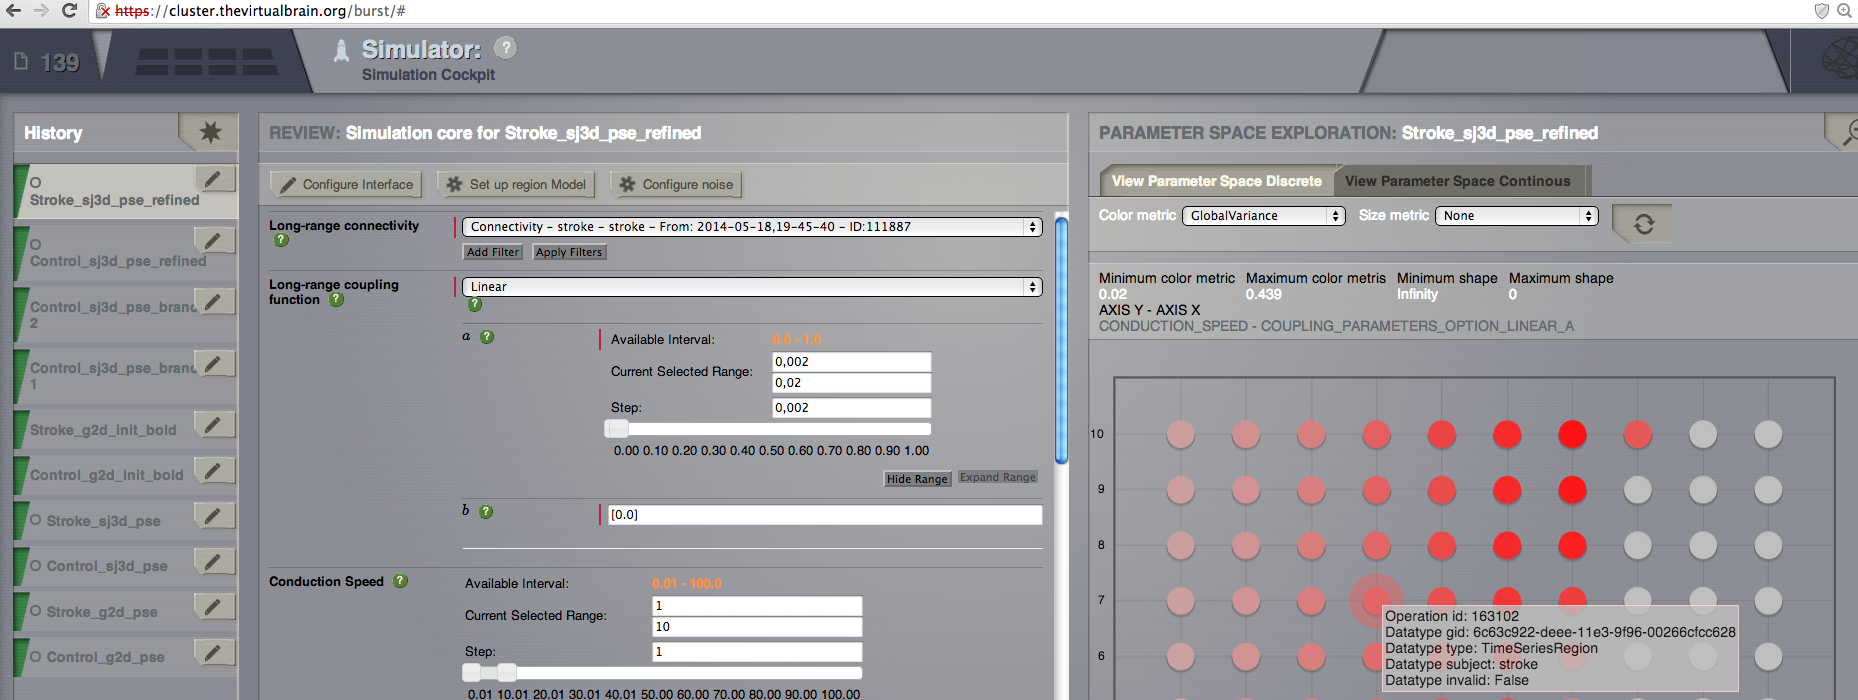
\includegraphics[width=0.82\linewidth]{Handout_UI_ModellingStructuralLesions_SelectPointFromPSE_a}
    \caption{Select points}
  \label{fig:steps_sim}
  \end{marginfigure}
  
  \begin{marginfigure}
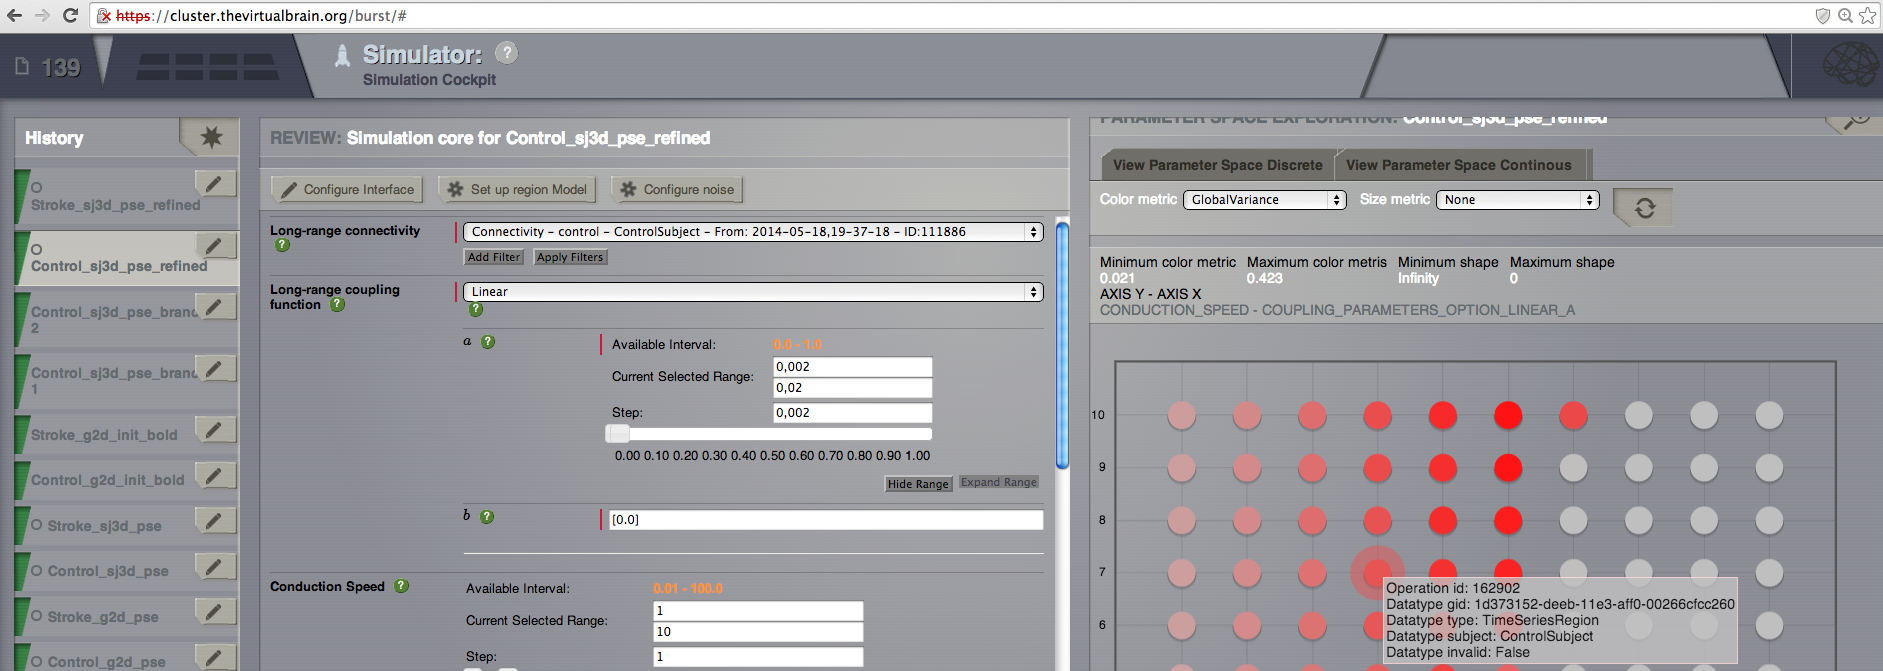
\includegraphics[width=0.82\linewidth]{Handout_UI_ModellingStructuralLesions_SelectPointFromPSE_b}
  \caption{Select points}
  \label{fig:steps_sim_03}
\end{marginfigure}

\begin{margintable}
  \centering
  \fontfamily{ppl}\selectfont
  \begin{tabular}{ll}
    \toprule
    Model parameter & Value \\
    \midrule
             $r$   & 0.006 \\
             $a$          &   1   \\
             $b$          &  3    \\
             $c$          &   1        \\
             $d$          &   5    \\
             $s$          &   4    \\
             $x_0$        &   -1.6        \\
             $K_{11}$     &   0.5        \\
             $K_{12}$     &   0.15     \\
             $K_{21}$     &   0.15       \\
             $\sigma$     &   0.3   \\
             $\mu$        &   3.3 \\
    \bottomrule
  \end{tabular}
  \caption{Stefanescu-Jirsa 3D parameters}
  \label{tab:modeltab}
\end{margintable}


  \begin{simulation}
  \begin{enumerate}
  \item Here, we will use the Stefanescu-Jirsa 3D (sj3d) presented in the previous talk. 
  \item Select the \textbf{control connectivity}, \textbf{long range linear coupling} with \underline{a range} between \textbf{0.002} and \textbf{0.02}, step \textbf{0.002}. Set the \underline{conduction speed} in the range \textbf{\unitfrac[1]{mm}{ms}} and \textbf{\unitfrac[10]{mm}{ms}}, step \textbf{\unitfrac[1]{mm}{ms}}.
  \item The model parameters are specified in Table \ref{tab:modeltab}. 
  \item In \underline{Variables watched by monitors} select only \textbf{xi}.
  \item The integration scheme is \textbf{HeunDeterministic} with \textbf{dt}$\mathbf{=}$\textbf{\unit[0.01]{ms}}.
  \item Launch two PSEs. The results are shown in Figs. \ref{fig:sj3d_control} and \ref{fig:sj3d_stroke} and correspond to simulations
  \textit{Control\_sj3d\_pse} and \textit{Stroke\_sj3d\_pse}.
  \item Select the point corresponding to a \underline{speed} of \textbf{\unitfrac[7]{mm}{ms}} and \underline{linear coupling strength} of \textbf{a=0.008} from each PSE map. Tag the corresponding time-series with \underline{Tag 2}: \textbf{sj3d} and \underline{Tag 3}: \textbf{A}. 
   \end{enumerate}
\end{simulation}



\begin{marginfigure}%
  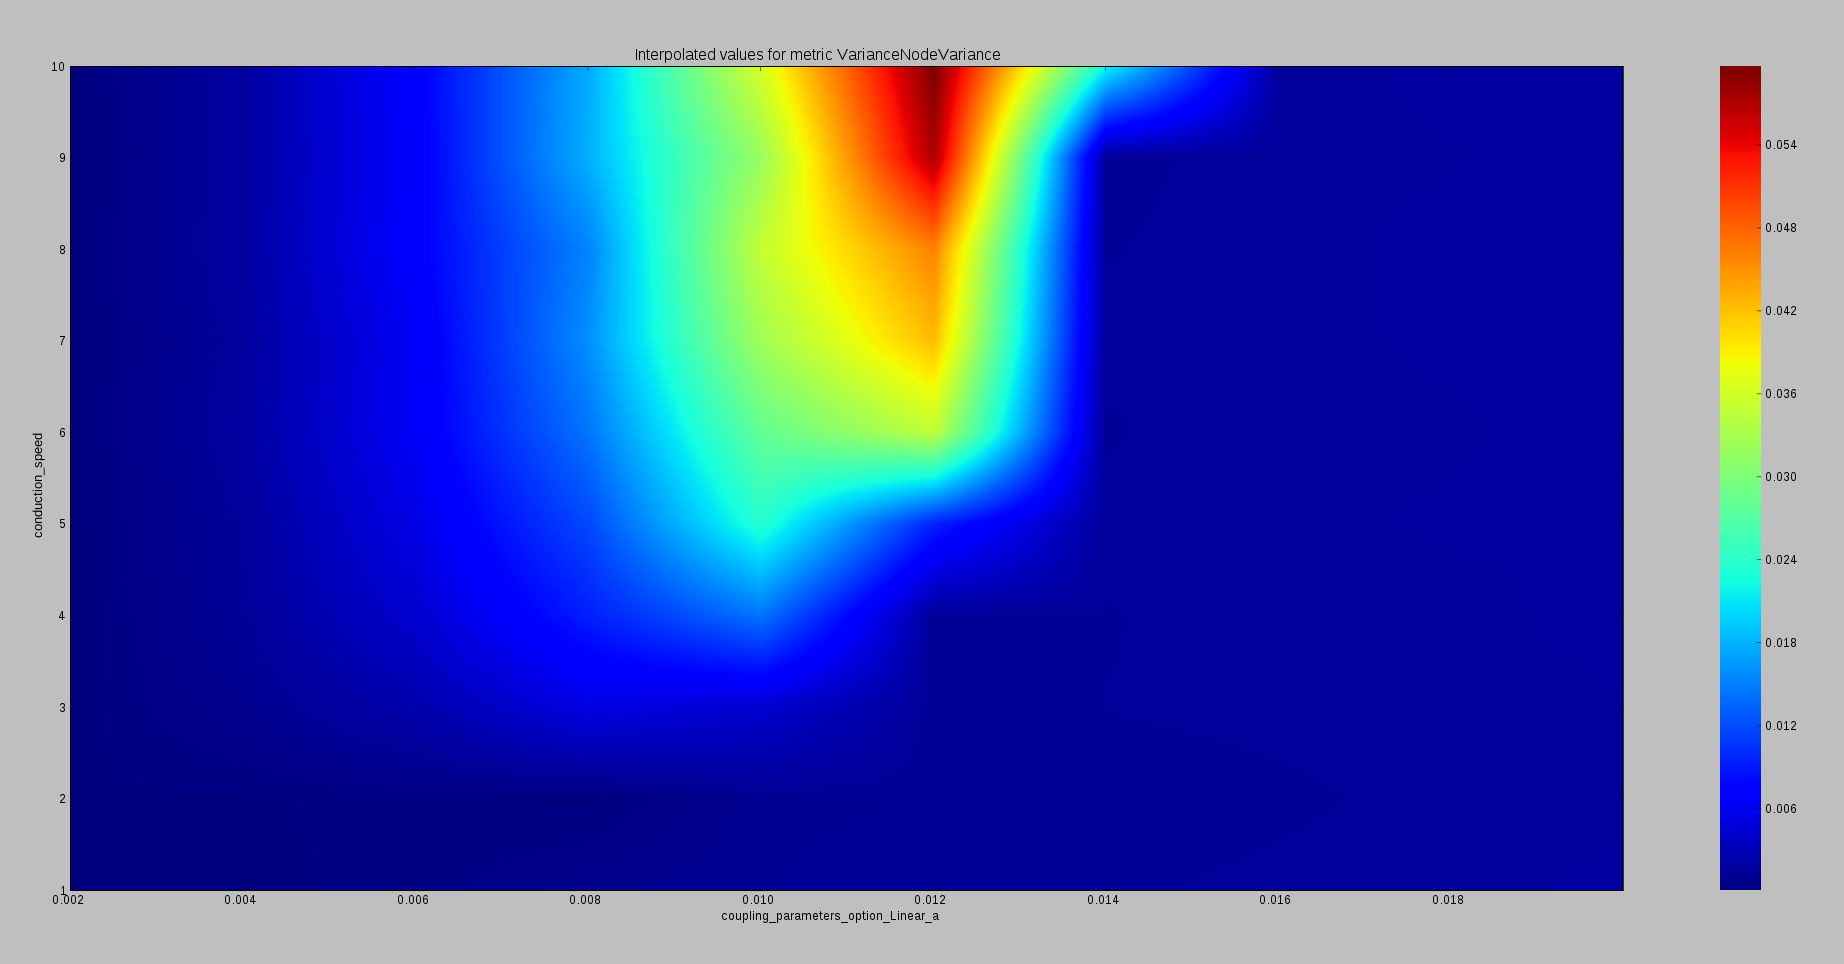
\includegraphics[width=0.82\linewidth]{Handout_UI_ModellingStructuralLesions_ControlSJ3DPSE}
    \caption{Variance map of \textit{Control\_sj3d\_pse}.}
  \label{fig:sj3d_control}
  \end{marginfigure}
  
  \begin{marginfigure}
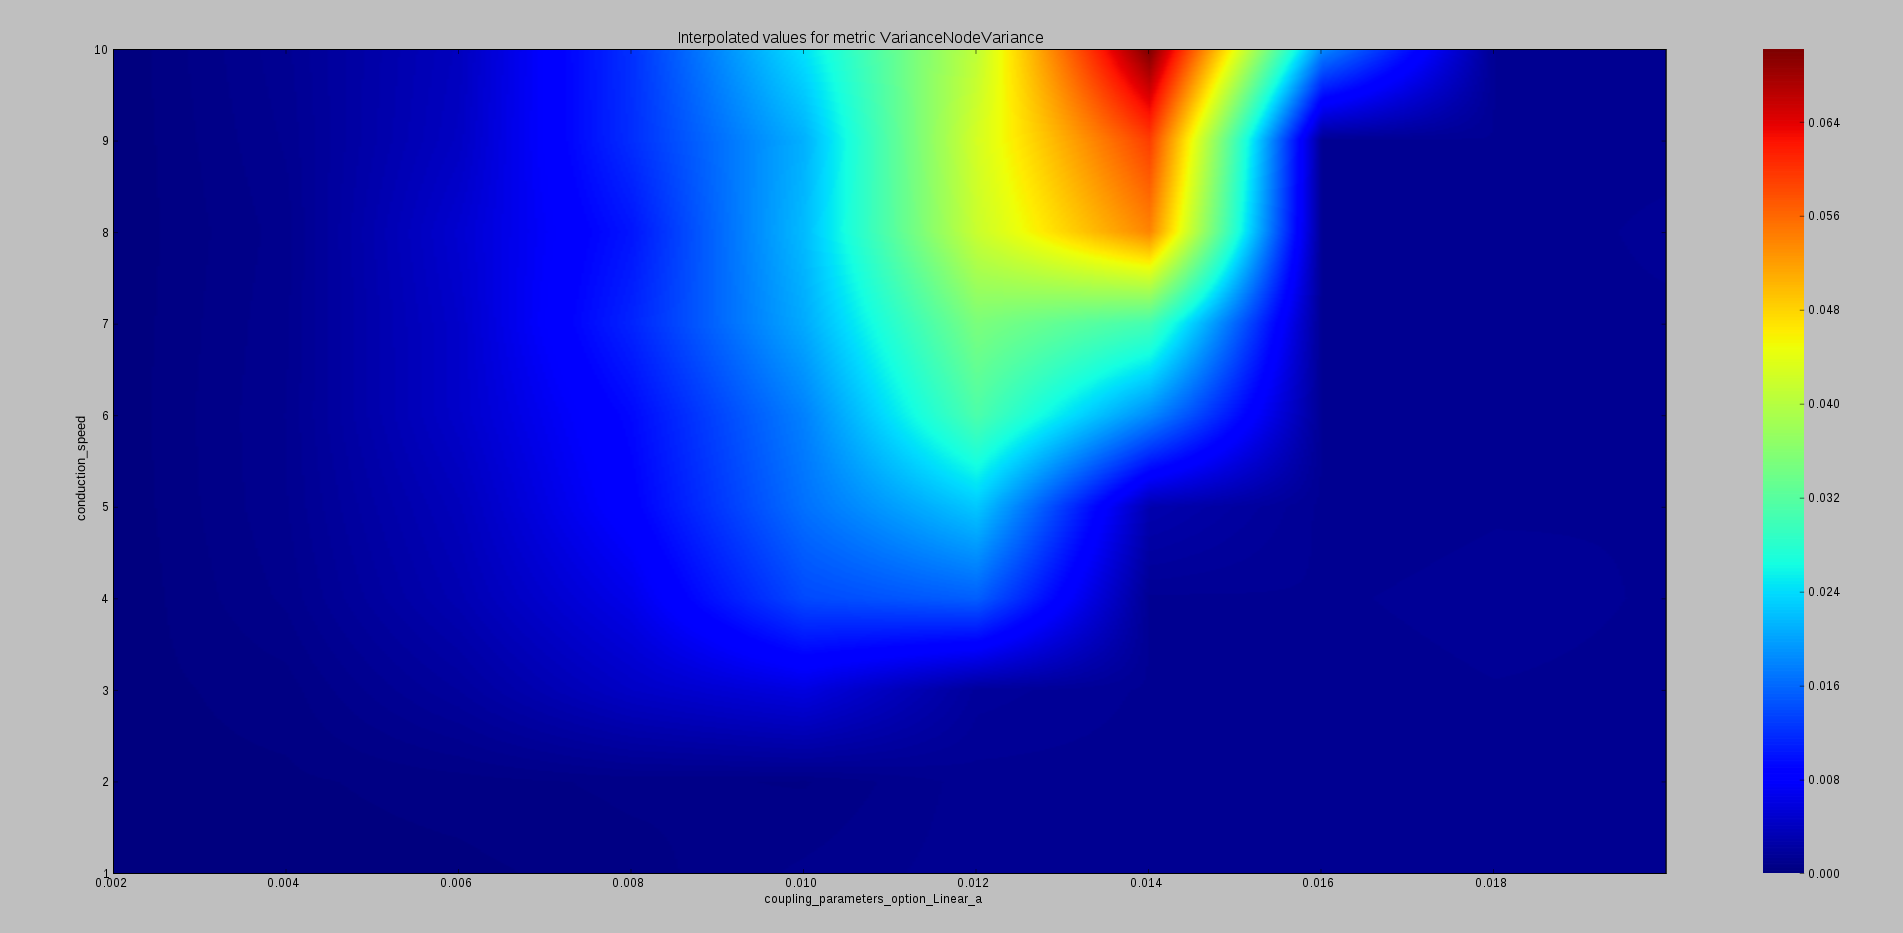
\includegraphics[width=0.82\linewidth]{Handout_UI_ModellingStructuralLesions_StrokeSJ3DPSE}
  \caption{Variance map of \textit{Stroke\_sj3d\_pse}.}
  \label{fig:sj3d_stroke}
\end{marginfigure}


\begin{simulation}
\begin{enumerate}[resume]
\setcounter{enumi}{7}
  \item Then, using the parameters from the previously tagged points, launch two \textbf{\unit[60]{s}} long simulations. This time, in addition to the variable \textbf{xi}, select also the variable \textbf{alpha}.
  \item  Use the \textbf{BOLD monitor} and the \textbf{Mixture of Gammas} \underline{HRF kernel} with its default parameters. The \underline{sampling period} of the monitor is \textbf{\unit[2000]{ms}}. 
\end{enumerate}
\end{simulation} 

These two simulations are not included in this project, but you will need them if you want to reproduce the simulations that are described below. 

\begin{simulation}
\begin{enumerate}[resume]
\setcounter{enumi}{9}
  \item Using the branching mechanism, launch \textbf{\unit[4]{min}} simulations from the two previous ones. These are \textit{Control\_sj3d\_init\_bold\_branch1} and \textit{Stroke\_sj3d\_init\_bold\_branch1}.
  \end{enumerate}
\end{simulation}

\newpage

\begin{formal}
\begin{enumerate}[resume]
\setcounter{enumi}{10}
\item Go to From \textsc{projects}$\rightarrow$ \textsc{Operation dashboard} compute the Pearson correlation coefficients matrix of the resulting spatially averaged time-series. 
  \end{enumerate}
\end{formal}

\begin{marginfigure}%
  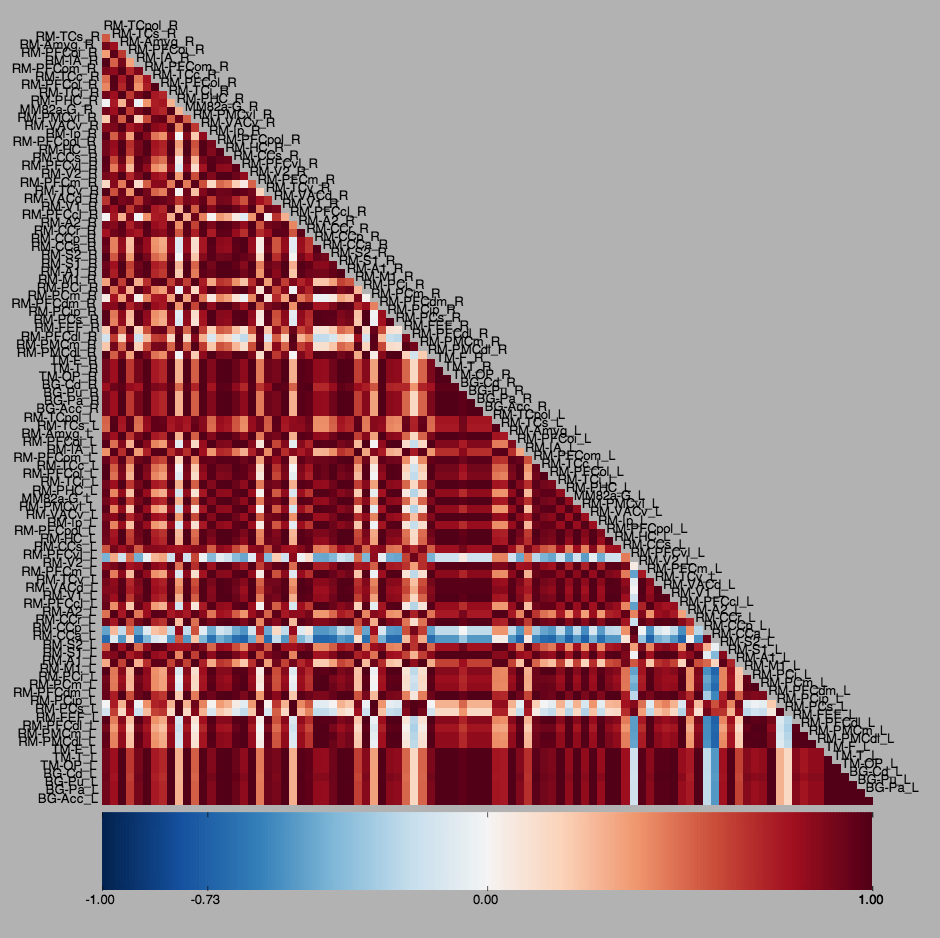
\includegraphics[width=\linewidth]{Handout_UI_ModellingStructuralLesions_bold_pearson_g2d_control.png}
  \caption{Pair-wise Pearson correlation coefficient matrix computed over the long BOLD time-series. Control matrix. }
  \label{fig:last}
  \end{marginfigure}
  \begin{marginfigure}
  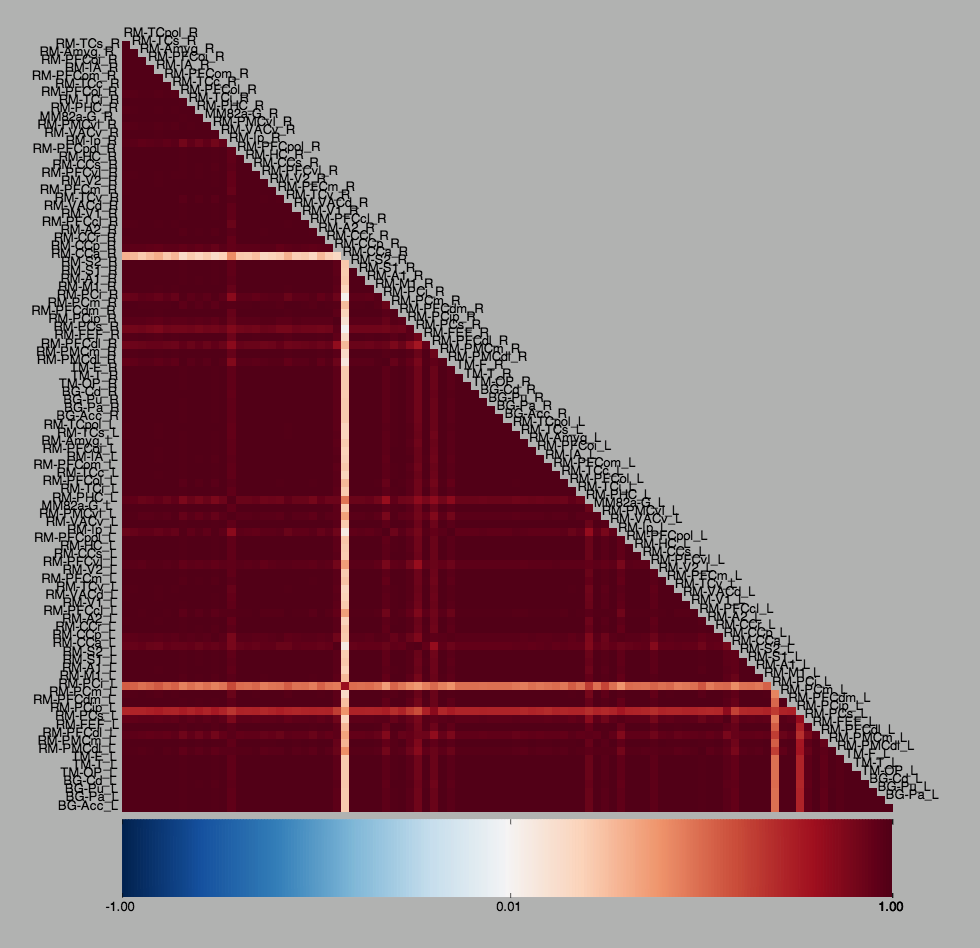
\includegraphics[width=\linewidth]{Handout_UI_ModellingStructuralLesions_bold_pearson_g2d_stroke.png}	
  \caption{Pair-wise Pearson correlation coefficient matrix computed over the long BOLD time-series. Stroke matrix.}
  \label{fig:steps_sim_07}
\end{marginfigure}

\begin{blah}
The region pair-wise Pearson correlation coefficients matrix is commonly referred to as to functional connectivity. It is often computed from BOLD time series. Here, for simplicity and comparative purpose we compute the matrix using spatially averaged time-series of neural activity. The results are exhibited in Figs. \ref{fig:last} and \ref{fig:steps_sim_07}.
\end{blah}

\section{More Documentation}\label{sec:more-doc}
For peer reviewed documentation on the software The Virtual Brain, please see the following articles \citep{Sanz-Leon_2013,  Woodman_2014}


\section{Support}\label{sec:support}

The official TVB webiste is \url{www.thevirtualbrain.org}.  
All the documentation and tutorials are hosted on \url{the-virtual-brain.github.io}.
You'll find our public \smallcaps{git} repository at \url{https://github.com/the-virtual-brain}. 
For questions and bug reports we have a users group \url{https://groups.google.com/forum/#!forum/tvb-users}

\bibliography{tvb_references}
\bibliographystyle{plainnat}

\end{document}